% ******************************* PhD Thesis Template **************************
% Please have a look at the README.md file for info on how to use the template

\documentclass[a4paper,12pt,times,numbered,print,index]{Classes/PhDThesisPSnPDF}

% ******************************************************************************
% ******************************* Class Options ********************************
% *********************** See README for more details **************************
% ******************************************************************************

% `a4paper'(The University of Cambridge PhD thesis guidelines recommends a page
% size a4 - default option) or `a5paper': A5 Paper size is also allowed as per
% the Cambridge University Engineering Deparment guidelines for PhD thesis
%
% `11pt' or `12pt'(default): Font Size 10pt is NOT recommended by the University
% guidelines
%
% `oneside' or `twoside'(default): Printing double side (twoside) or single
% side.
%
% `print': Use `print' for print version with appropriate margins and page
% layout. Leaving the options field blank will activate Online version.
%
% `index': For index at the end of the thesis
%
% `draftclassic': For draft mode without loading any images (same as draft in book)
%
% `draft': Special draft mode with line numbers, images, and water mark with
% timestamp and custom text. Position of the text can also be modified.
%
% `abstract': To generate only the title page and abstract page with
% dissertation title and name, to submit to the Student Registry
%
% `chapter`: This option enables only the specified chapter and it's references
%  Useful for review and corrections.
%
% ************************* Custom Page Margins ********************************
%
% `custommargin`: Use `custommargin' in options to activate custom page margins,
% which can be defined in the preamble.tex. Custom margin will override
% print/online margin setup.
%
% *********************** Choosing the Fonts in Class Options ******************
%
% `times' : Times font with math support. (The Cambridge University guidelines
% recommend using times)
%
% `fourier': Utopia Font with Fourier Math font (Font has to be installed)
%            It's a free font.
%
% `customfont': Use `customfont' option in the document class and load the
% package in the preamble.tex
%
% default or leave empty: `Latin Modern' font will be loaded.
%
% ********************** Choosing the Bibliography style ***********************
%
% `authoryear': For author-year citation eg., Krishna (2013)
%
% `numbered': (Default Option) For numbered and sorted citation e.g., [1,5,2]
%
% `custombib': Define your own bibliography style in the `preamble.tex' file.
%              `\RequirePackage[square, sort, numbers, authoryear]{natbib}'.
%              This can be also used to load biblatex instead of natbib
%              (See Preamble)
%
% **************************** Choosing the Page Style *************************
%
% `default (leave empty)': For Page Numbers in Header (Left Even, Right Odd) and
% Chapter Name in Header (Right Even) and Section Name (Left Odd). Blank Footer.
%
% `PageStyleI': Chapter Name next & Page Number on Even Side (Left Even).
% Section Name & Page Number in Header on Odd Side (Right Odd). Footer is empty.
%
% `PageStyleII': Chapter Name on Even Side (Left Even) in Header. Section Number
% and Section Name in Header on Odd Side (Right Odd). Page numbering in footer


% ********************************** Preamble **********************************
% Preamble: Contains packages and user-defined commands and settings
% ******************************************************************************
% ****************************** Custom Margin *********************************

% Add `custommargin' in the document class options to use this section
% Set {innerside margin / outerside margin / topmargin / bottom margin}  and
% other page dimensions
\ifsetCustomMargin
  \RequirePackage[left=37mm,right=30mm,top=35mm,bottom=30mm]{geometry}
  \setFancyHdr % To apply fancy header after geometry package is loaded
\fi

% Add spaces between paragraphs
%\setlength{\parskip}{0.5em}
% Ragged bottom avoids extra whitespaces between paragraphs
\raggedbottom
% To remove the excess top spacing for enumeration, list and description
%\usepackage{enumitem}
%\setlist[enumerate,itemize,description]{topsep=0em}

% *****************************************************************************
% ******************* Fonts (like different typewriter fonts etc.)*************

% Add `customfont' in the document class option to use this section

\ifsetCustomFont
  % Set your custom font here and use `customfont' in options. Leave empty to
  % load computer modern font (default LaTeX font).
  %\RequirePackage{helvet}

  % For use with XeLaTeX
  %  \setmainfont[
  %    Path              = ./libertine/opentype/,
  %    Extension         = .otf,
  %    UprightFont = LinLibertine_R,
  %    BoldFont = LinLibertine_RZ, % Linux Libertine O Regular Semibold
  %    ItalicFont = LinLibertine_RI,
  %    BoldItalicFont = LinLibertine_RZI, % Linux Libertine O Regular Semibold Italic
  %  ]
  %  {libertine}
  %  % load font from system font
  %  \newfontfamily\libertinesystemfont{Linux Libertine O}
\fi

% *****************************************************************************
% **************************** Custom Packages ********************************

% ************************* Algorithms and Pseudocode **************************
\usepackage{algorithm}
\usepackage[noend]{algpseudocode}
\newcommand*\Let[2]{\State #1 $\gets$ #2}


% ********************Captions and Hyperreferencing / URL **********************

% Captions: This makes captions of figures use a boldfaced small font.
%\RequirePackage[small,bf]{caption}

\RequirePackage[labelsep=space,tableposition=top]{caption}
\renewcommand{\figurename}{Fig.} %to support older versions of captions.sty


% *************************** Graphics and figures *****************************

%\usepackage{rotating}
%\usepackage{wrapfig}

% Uncomment the following two lines to force Latex to place the figure.
% Use [H] when including graphics. Note 'H' instead of 'h'
%\usepackage{float}
%\restylefloat{figure}

% Subcaption package is also available in the sty folder you can use that by
% uncommenting the following line
% This is for people stuck with older versions of texlive
%\usepackage{sty/caption/subcaption}
\usepackage{subcaption}

% ********************************** Tables ************************************
\usepackage{booktabs} % For professional looking tables
\usepackage{multirow}

%\usepackage{multicol}
%\usepackage{longtable}
%\usepackage{tabularx}


% *********************************** SI Units *********************************
\usepackage{siunitx} % use this package module for SI units
\newtheorem{mydef}{Definition}


%copied stuff for confusion matrix
\usepackage{tikz}
\usetikzlibrary{positioning}

%stuff for subfigures

%stuff for table caption

% ******************************* Line Spacing *********************************

% Choose linespacing as appropriate. Default is one-half line spacing as per the
% University guidelines

% \doublespacing
% \onehalfspacing
% \singlespacing


% ************************ Formatting / Footnote *******************************

% Don't break enumeration (etc.) across pages in an ugly manner (default 10000)
%\clubpenalty=500
%\widowpenalty=500

%\usepackage[perpage]{footmisc} %Range of footnote options


% *****************************************************************************
% *************************** Bibliography  and References ********************

%\usepackage{cleveref} %Referencing without need to explicitly state fig /table

% Add `custombib' in the document class option to use this section
\ifuseCustomBib
   \RequirePackage[square, sort, numbers, authoryear]{natbib} % CustomBib

% If you would like to use biblatex for your reference management, as opposed to the default `natbibpackage` pass the option `custombib` in the document class. Comment out the previous line to make sure you don't load the natbib package. Uncomment the following lines and specify the location of references.bib file

%\RequirePackage[backend=biber, style=numeric-comp, citestyle=numeric, sorting=nty, natbib=true]{biblatex}
%\bibliography{References/references} %Location of references.bib only for biblatex

\fi

% changes the default name `Bibliography` -> `References'
\renewcommand{\bibname}{References}


% ******************************** Roman Pages *********************************
% The romanpages environment set the page numbering to lowercase roman one
% for the contents and figures lists. It also resets
% page-numbering for the remainder of the dissertation (arabic, starting at 1).

\newenvironment{romanpages}{
  \setcounter{page}{1}
  \renewcommand{\thepage}{\roman{page}}}
{\newpage\renewcommand{\thepage}{\arabic{page}}}


% ******************************************************************************
% ************************* User Defined Commands ******************************
% ******************************************************************************

% *********** To change the name of Table of Contents / LOF and LOT ************

%\renewcommand{\contentsname}{My Table of Contents}
%\renewcommand{\listfigurename}{My List of Figures}
%\renewcommand{\listtablename}{My List of Tables}


% ********************** TOC depth and numbering depth *************************

\setcounter{secnumdepth}{2}
\setcounter{tocdepth}{2}


% ******************************* Nomenclature *********************************

% To change the name of the Nomenclature section, uncomment the following line

%\renewcommand{\nomname}{Symbols}


% ********************************* Appendix ***********************************

% The default value of both \appendixtocname and \appendixpagename is `Appendices'. These names can all be changed via:

%\renewcommand{\appendixtocname}{List of appendices}
%\renewcommand{\appendixname}{Appndx}

% *********************** Configure Draft Mode **********************************

% Uncomment to disable figures in `draftmode'
%\setkeys{Gin}{draft=true}  % set draft to false to enable figures in `draft'

% These options are active only during the draft mode
% Default text is "Draft"
%\SetDraftText{DRAFT}

% Default Watermark location is top. Location (top/bottom)
%\SetDraftWMPosition{bottom}

% Draft Version - default is v1.0
%\SetDraftVersion{v1.1}

% Draft Text grayscale value (should be between 0-black and 1-white)
% Default value is 0.75
%\SetDraftGrayScale{0.8}


% ******************************** Todo Notes **********************************
%% Uncomment the following lines to have todonotes.

%\ifsetDraft
%	\usepackage[colorinlistoftodos]{todonotes}
%	\newcommand{\mynote}[1]{\todo[author=kks32,size=\small,inline,color=green!40]{#1}}
%\else
%	\newcommand{\mynote}[1]{}
%	\newcommand{\listoftodos}{}
%\fi

% Example todo: \mynote{Hey! I have a note}


% ************************ Thesis Information & Meta-data **********************
% Thesis title and author information, refernce file for biblatex
% ************************ Thesis Information & Meta-data **********************
%% The title of the thesis
\title{Semantic Complex Pattern Mining on Event Streams}
%\texorpdfstring is used for PDF metadata. Usage:
%\texorpdfstring{LaTeX_Version}{PDF Version (non-latex)} eg.,
%\texorpdfstring{$sigma$}{sigma}

%% The full name of the author
\author{Leon Bornemann}

%% Department (eg. Department of Engineering, Maths, Physics)
\dept{Department of Mathematics and Computer Science}

%% University and Crest
\university{Freie Universit\"at Berlin}
% Crest minimum should be 30mm.
\crest{
\includegraphics[width=0.4\textwidth]{FULogo}}
%% Use this crest, if you are using the college crest
%% Crest long miminum should be 65mm
%\crest{
\includegraphics[width=0.45\textwidth]{University_Crest_Long}}

%% College shield [optional] 
% Crest minimum should be 30mm.
%\collegeshield{
\includegraphics[width=0.2\textwidth]{CollegeShields/Kings}}


%% Supervisor (optional)
%\supervisor{Prof. Kenichi Soga}
%% Supervisor Role (optional) - Supervisor (default) or advisor
%\supervisorrole{Advisor: }

%% Advisor (optional)
%\advisor{Prof. Malcolm Bolton}
%% Advisor Role (optional) - Advisor (default) or leave empty
%\advisorrole{Advisor: }


%% You can redefine the submission text:
% Default as per the University guidelines:
% ``This dissertation is submitted for the degree of''
\renewcommand{\submissiontext}{This thesis is submitted for the degree of}

%% Full title of the Degree
\degreetitle{Master of Science}

%% College affiliation (optional)
%%\college{King's College}

%% Submission date
% Default is set as {\monthname[\the\month]\space\the\year}
%\degreedate{September 2014} 

%% Meta information
\subject{Data Stream Mining} \keywords{{Pattern Mining} {Data Stream} {Complex Event Mining} {Episode Discovery} {Prediction} }


% ***************************** Abstract Separate ******************************
% To printout only the titlepage and the abstract with the PhD title and the
% author name for submission to the Student Registry, use the `abstract' option in
% the document class.

\ifdefineAbstract
 \pagestyle{empty}
 \includeonly{Declaration/declaration, Abstract/abstract}
\fi

% ***************************** Chapter Mode ***********************************
% The chapter mode allows user to only print particular chapters with references
% Title, Contents, Frontmatter are disabled by default
% Useful option to review a particular chapter or to send it to supervisior.
% To use choose `chapter' option in the document class

\ifdefineChapter
 \includeonly{Chapter3/chapter3}
\fi

% ******************************** Front Matter ********************************
\begin{document}

\frontmatter

\begin{titlepage}
  \maketitle
\end{titlepage}


%% ******************************* Thesis Dedidcation ********************************

\begin{dedication} 

I would like to dedicate this thesis to my loving parents \dots

\end{dedication}


% ******************************* Thesis Declaration ***************************

\begin{declaration}

Does the FU have a declaration text in which I declare that I worked on this alone, up to scientific standard, did not copy anything without citing etc? If yes I will put this here.

% Author and date will be inserted automatically from thesis.tex \author \degreedate

\end{declaration}


% ************************** Thesis Acknowledgements **************************

\begin{acknowledgements}      


And I would like to acknowledge (TODO) ... 


\end{acknowledgements}

% ************************** Thesis Abstract *****************************
% Use `abstract' as an option in the document class to print only the titlepage and the abstract.
\begin{abstract}
It is a little early for an abstract, I guess I could already write a preliminary Abstract...
\end{abstract}


% *********************** Adding TOC and List of Figures ***********************

\tableofcontents

\listoffigures

\listoftables

% \printnomenclature[space] space can be set as 2em between symbol and description
%\printnomenclature[3em]

\printnomenclature

% ******************************** Main Matter *********************************
\mainmatter

%*******************************************************************************
%*********************************** First Chapter *****************************
%*******************************************************************************

\chapter{Introduction}  %Title of the First Chapter

\ifpdf
    \graphicspath{{Chapter1/Figs/Raster/}{Chapter1/Figs/PDF/}{Chapter1/Figs/}}
\else
    \graphicspath{{Chapter1/Figs/Vector/}{Chapter1/Figs/}}
\fi

This chapter serves as a rather broad introduction to the topic of this thesis and provides motivation for the work.

\section{General Introduction and Motivation}
Almost any application domain of information systems has some data that is being generated. Data is available in many different forms. One of these forms are data streams. Data streams are not limited to the recent rise in popularity of video and audio streams. On the contrary the application domains that produce data in the form of streams are very diverse. They include for example constantly running business applications that log business activities and events, sensor networks that report usage data or devices that take measurements of physical quantities (such as temperature, pressure, humidity, etc...) at certain points of time. \newline
The fact that streams generate a constant stream of data and thus lead to a constantly growing database is a significant difference to classic applications of data mining in which there is a static (training) database. Despite that significant difference, many fields of interest in the context of static databases are also of interest for data streams. These areas include frequent patterns, predictive patterns, association rules, clustering and classification of the data entities. Approaches and algorithms that solve these problems for static databases, while by no means fully researched, are rather well known and evaluated. Applying these methods to data streams can present challenges and may demand many modifications due to the large and possibly infinite amounts of data produced by streams. Naturally, data mining methods for stream data must be especially fast, scalable and memory efficient. \newline
Apart from the additional, algorithmic constraints on memory and computation time, data streams also present conceptual challenges. In contrast to static databases streams may evolve over time, which can make it very difficult for algorithms to assess which past data of the stream should be considered when analyzing the currently incoming data. Recognizing these so called concept drifts is one challenge among many when processing or mining data streams. \newline
A suitable way to look at most data streaming scenarios is that of event streams. An event can be basically anything that happens in the real world, represented as an element of a data stream. Examples of this could be a rise in temperature that is reported by a sensor or an increase in the value of a stock, that is being traded at a stock market. These events are commonly referred to as basic or simple events. \newline
This thesis attempts to combine two research areas that are of interest in event streams: Complex Event Mining and Prediction. Complex events are structures that consist of multiple basic events with different relationships between each other. Discovering interesting complex event patterns can be tough, especially since there may be a lot of potential candidates. The discovery of complex events is related to the research area of pattern mining, since complex events are essentially large patterns, that are mined from basic events. Traditionally, pattern mining is often employed to extract knowledge or interesting correlations. The prediction of certain events in an ongoing event stream has many obvious use cases such as building early warning systems for hazardous events like power outages in power grids, failures in sensor networks or even natural disasters, such as earthquakes. \\
The idea to combine these two research area is rather simple. We aim to mine complex events from an event stream with the specific purpose of predicting future occurrences of a specific event type. When mining complex events we also want to consider semantic knowledge in addition to the data present in the stream. If the semantic knowledge about the underlying event stream contains information about the different event types it is possible to use that knowledge directly in the mining process. Semantic knowledge can take many different forms, a common one being an RDF-graph that can be examined using queries. \newline
Figure \ref{fig_approach} summarizes the basic idea of this thesis graphically. The underlying event stream is mined for complex events by a mining algorithm that will consider the information given in the stream as well as the semantic knowledge. The resulting complex events are then used as input for a model building algorithm, which will produce a predictive model.
\begin{figure}[h]
	\centering
  	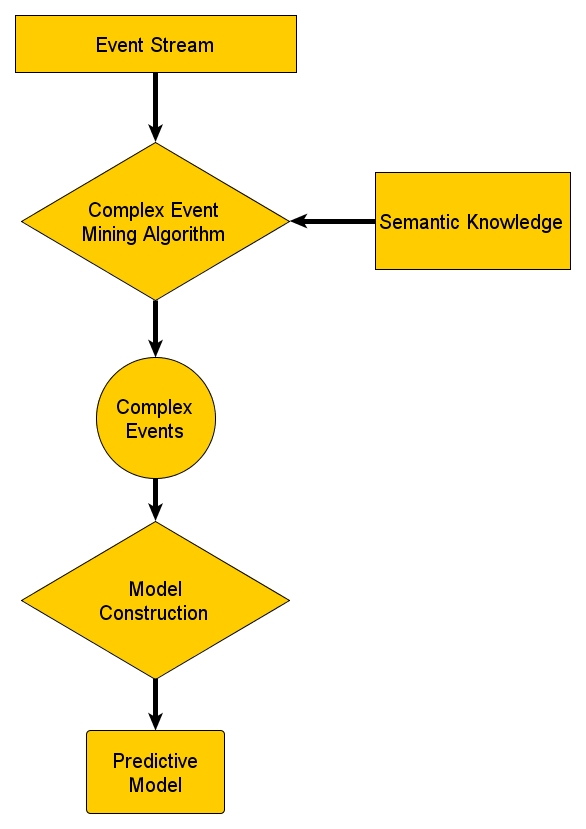
\includegraphics[width=0.5\textwidth]{approach.jpg}
	\caption{General Structure of the approach suggested by this thesis.}
	\label{fig_approach}
\end{figure}

In terms of the very broad term of complex events this thesis will focus on the subtopic of episode pattern mining. Episodes are a specific kind of complex events and are formally defined in chapter \ref{chapter_related}. For now it is sufficient to know that episodes are essentially complex events in which single events or entire episodes can be combined using two operators: the conjunction and the sequence operator. Figure \ref{fig_simpleEpisodeExample} visualizes a simple episode pattern and example occurrences in a data stream.

\begin{figure}[h]
	\centering
  	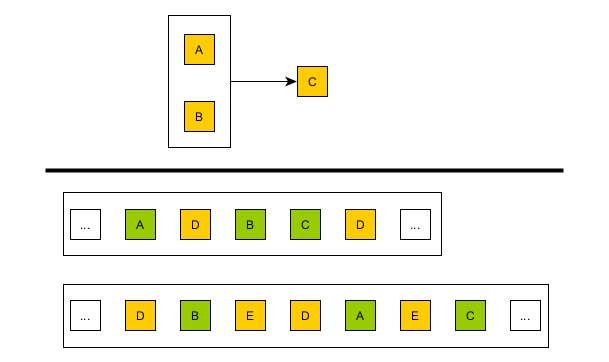
\includegraphics[width=0.5\textwidth]{exampleEpisode.jpg}
	\caption{The top half visualizes an example episode pattern, which consist of a conjunction (A and B must both occur, but the order does not matter) and a sequence (C must occur after A and B). The bottom half shows two windows of an example stream, in which occurrences of the episode are shown in green.}
	\label{fig_simpleEpisodeExample}
\end{figure}

Episodes are sequential patterns that have previously been mined from very long sequences, which makes them an appropriate mining target in event streams, since streams and sequences share the sequential nature. The only difference is that streams grow over time, whereas sequences have a fixed size.\\
%Instead of just analyzing all frequent episodes, this thesis will focus on finding predictive episodes, meaning episodes which can help to predict events occurring in the future. As already mentioned prediction of events is a highly relevant application area, since the potential benefits of well performing models are enormous.
The domain that will be used in the evaluation of this thesis is stock market prediction. Both predicting the overall direction of the stock market and predicting whether individual stocks will rise or fall are a difficult problems that have the obvious application of making profitable investments. \newline
The rest of the thesis is outlined as follows: Chapter \ref{chapter_related} introduces the basic terminology and reviews the related work, Chapter \ref{chapter_background} follows up with formal definitions and a more detailed introduction to episode mining. Chapter \ref{chapter_solutions} presents the suggested algorithms to mine predictive models for event streams using episodes and analyzes their complexities. Subsequently chapter \ref{chapter_evaluation} presents an extensive evaluation using real stock market data. Finally chapter \ref{chapter_conclusion} concludes the paper and mentions possible future work.


%TODO use this somewhere
%In contrast to other regression and forecasting methods, such as artificial neural networks, predictive episodes have the advantage that once they are discovered they can make ad-hoc predictions in a fast moving data-stream, whereas neural networks usually forecast the closing values of stock markets of the next day based on the values of previous days. This gives predictive episodes a niche: fast moving (real-time) data-streams that need quick predictions of future events. \newline

\section{Problem Definition and Exact Research Question}
Even though many terms have not yet been precisely defined (which will be done in chapter \ref{chapter_related} ) this section presents a loose, intuitive definition of the problem to be tackled by this thesis. Given a stream of basic events and a special event type $P$ one is interested to predict occurrences of that special event type $P$ in the stream, so that actions can be taken before $P$ actually occurs. For this purpose we are interested to discover episodes in the stream of which occurrences are temporally correlated to the occurrence of $P$. A window of an example stream is visualized in figure \ref{fig_predictiveEpisodeExample}. In this simple example the episode $A$ followed by $E$ always occurs before $P$.

\begin{figure}[h]
	\centering
  	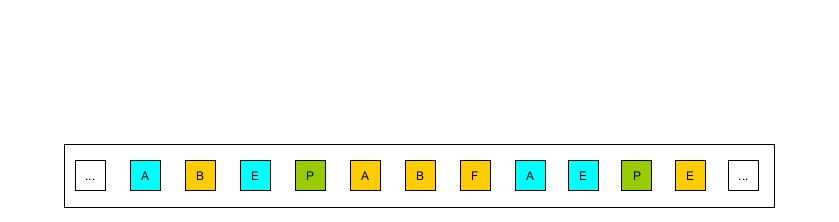
\includegraphics[width=0.6\textwidth]{examplePrediction.jpg}
	\caption{The figure visualizes an event stream in which events of type $P$ are to be predicted. The occurrences of the episode $A$ followed by $E$ is colored in teal, whereas events of types $P$ are colored in green and all other events are yellow}
	\label{fig_predictiveEpisodeExample}
\end{figure}

Note that it is very important to the mining process how much time is allowed to pass between the occurrence of the mined episode and the event that is to predict. If this time span is too small a mining algorithm might not find reliable correlations. If the timespan is too large a mining algorithm might be overwhelmed by the number of candidates that need to be considered, since the more time may pass the larger are the sequences before each event $P$ that must be considered. %TODO maybe move the last sentences to method? 
\newline
To solve the problem outlined above a semantic mining algorithm will be suggested in this thesis. Since the underlying data structure to be analyzed are data streams, the algorithm must have the following properties:
\begin{itemize}
	\item The algorithm must be able to adapt to a changing context (as the stream progresses, the underlying correlation may change completely)
	\item The recognition of episodes must be quick, since streams, especially in the domain of stock markets, can have a high velocity. This makes it important to be able to quickly predict events. If the prediction takes too long, the event which we want to predict may have already occurred before the algorithm outputs its prediction, thus robbing the user of the opportunity to take action.
	\item The Algorithm must not require to store the entire stream of events seen so far, since that is not feasible for most streams.
\end{itemize}

The algorithm will be evaluated on real-life data-sets from the domain of stock market prediction, in which the developed algorithm will be empirically compared to other approaches in terms of accuracy measures and execution time. In summary the research question in particular is:\newline \newline
\textbf{How can event streams be mined for episodes that help predict certain event types and how can domain knowledge be used to improve the results of the mining algorithm?}
%*******************************************************************************
%****************************** Second Chapter *********************************
%*******************************************************************************

\chapter{Related Work}
\label{chapter_related}

\ifpdf
    \graphicspath{{Chapter2/Figs/Raster/}{Chapter2/Figs/PDF/}{Chapter2/Figs/}}
\else
    \graphicspath{{Chapter2/Figs/Vector/}{Chapter2/Figs/}}
\fi

This chapter reviews the related work relevant for this thesis. Since there are many different related work areas that all have their relevance to this thesis, this chapter is divided into different sections dealing with each of them in turn. First section \ref{sec_basicDefinitions} introduces and defines basic the basic terminology that will be used in this thesis. Afterwards section \ref{sec_streamMining} gives a broad overview over the general area of mining data streams but lays a focus on the mining patterns as well as prediction algorithms especially for the domain of financial data. Subsequently section \ref{sec_episodes} briefly introduces the concept of episodes and summarizes the related work for episode mining. Finally section TODO concludes with a brief overview over semantic technologies.

\section{Basic Definitions and Terminology}
\label{sec_basicDefinitions}
The basic terminology in this subsection is paraphrased from the event processing glossary created by the Event Processing Technical Society \cite{luckham2011epts}. Note that some of the definitions may be slightly altered or simplified. This is due to the fact that the event processing technical society uses these terms for a very general description of event processing and event processing architectures and thus some original definitions are more complex than what is needed in this thesis. The definitions given here aim to establish a clear terminology for this thesis.

\begin{mydef}
\textbf{Event} An event is either something that is happening in the real world or in the context of computer science an object that represents a real world event and records its properties. The latter can also be referred to as an event object or an event tuple. Note that the term is overloaded, but the context usually gives a clear indication of what is meant.
\end{mydef}

The event processing society claims that the context usually solves the ambiguity in the above definition. Since this may not always be the case we will only use the term \textit{event} in this thesis to refer to event objects unless it is otherwise specified.

\begin{mydef}
\textbf{Simple Event} A simple event is an event that is not viewed as summarizing, representing, or denoting a set of other events. Sometimes also referred to as a basic events.
\end{mydef}

These two definitions can sometimes cause confusion. It is important to note that the term event is the most general term, since it can refer to any kind of event, be it simple, derived or complex (see definitions \ref{def_derivedEvent} and \ref{def_complexEvent}). A simple event however is the most basic form of an event and often the ingredient for the creation of more complex events:
Given simple events it is possible to derive events from those or the absence of those. For example the absence measurement events of a sensor could be used to derive the event of that very same sensor becoming defect. These events are called derived events:

\begin{mydef}
\label{def_derivedEvent}
\textbf{Derived Event} A derived event or synthesized event is an event that is generated according to some method or based on some reasoning process.
\end{mydef}

It is also possible to combine multiple simple events to form what we refer to as complex events:

\begin{mydef}
\label{def_complexEvent}
\textbf{Complex Event} A complex event is a derived event that is created by combining other events. The events can be combined by using certain operators, for example disjunction, conjunction or sequence. An example would be $(A \land B) \rightarrow C$ (event A and B in any order followed by event C).
\end{mydef}

This is a very broad definition of complex events. The choice of allowed operators strongly impacts the expressiveness of complex events. A specific kind of complex events are episodes (see section \ref{sec_episodes}), which will be the main focus of this thesis.
The next notion that needs to be considered is that each individual event normally belongs to a certain class of events, which we refer to as the event type:

\begin{mydef}
\textbf{Event type} The event type, sometimes also referred to as event class, event definition, or event schema is a label that identifies events as members of an event class.
\end{mydef}

Another important term that was not explicitly defined in the event processing glossary, but is very relevant to the topic at hand is the notion of a type alphabet:

\begin{mydef}
\textbf{Type Alphabet} The type alphabet, often simply called the event alphabet, is the set of all possible event types that can occur in the observed system.
\end{mydef}

Event alphabets are often implicitly defined when mining frequent itemsets, patterns or episodes.
So far we have looked at events without considering the scenario we are most interested in which are event streams. To do so we need the notion of timestamps:

\begin{mydef}
\textbf{Timestamp} A time value of an event indicating its creation or arrival time.
\end{mydef}

Given that we can define an event stream:

\begin{mydef}
\textbf{Event Stream} An event stream is an ordered sequence of events, usually ordered by the event timings.
\end{mydef}

Note that this rather broad definition of an event stream does not assume anything about the kind of event that is contained in it. A stream can contain very basic forms of events (simple events) but can also be made up out of derived events or even complex events. Also other properties for example that the stream is constantly updating (new events coming in) are not considered yet.


\section{Data Stream Mining}
\label{sec_streamMining}
As already mentioned in the introduction data streams present a challenge to data miners in many ways. This section aims to give both a general overview over the broad research area of mining data stream as well as specifically cover the related topics of pattern mining and prediction (forecasting). \\

\subsection{Taxonomy of the Research Areas}
First of all it is useful to note that many research areas in classical data mining are also of interest when processing streams. As already mentioned in the introduction however, data streams impose severe restrictions on the algorithms, such as them having to use only one pass over the data and that they should be incremental. Most data mining algorithms for the classical scenario in which the underlying data is a static database do not satisfy these properties. Thus the algorithms need to be modified and often approximations have to be made. A comprehensive, basic overview over the application of different data mining tasks and how they can be applied to streams was comprised by Gaber et. al. \cite{gaber2005mining}. Note that the paper by Gaber et. al. was published in 2005, so quite a lot of work has been done since then, which means that these papers are obviously not present in their literature review. However the overview provided by the authors is still very useful, since it brings structure to the large field of data stream mining. A taxonomy that follows the basic structure of the paper by Gaber et. al. is visualized in figure \ref{fig_streamMiningTaxonomy}.

\begin{figure}[h]
	\centering
  	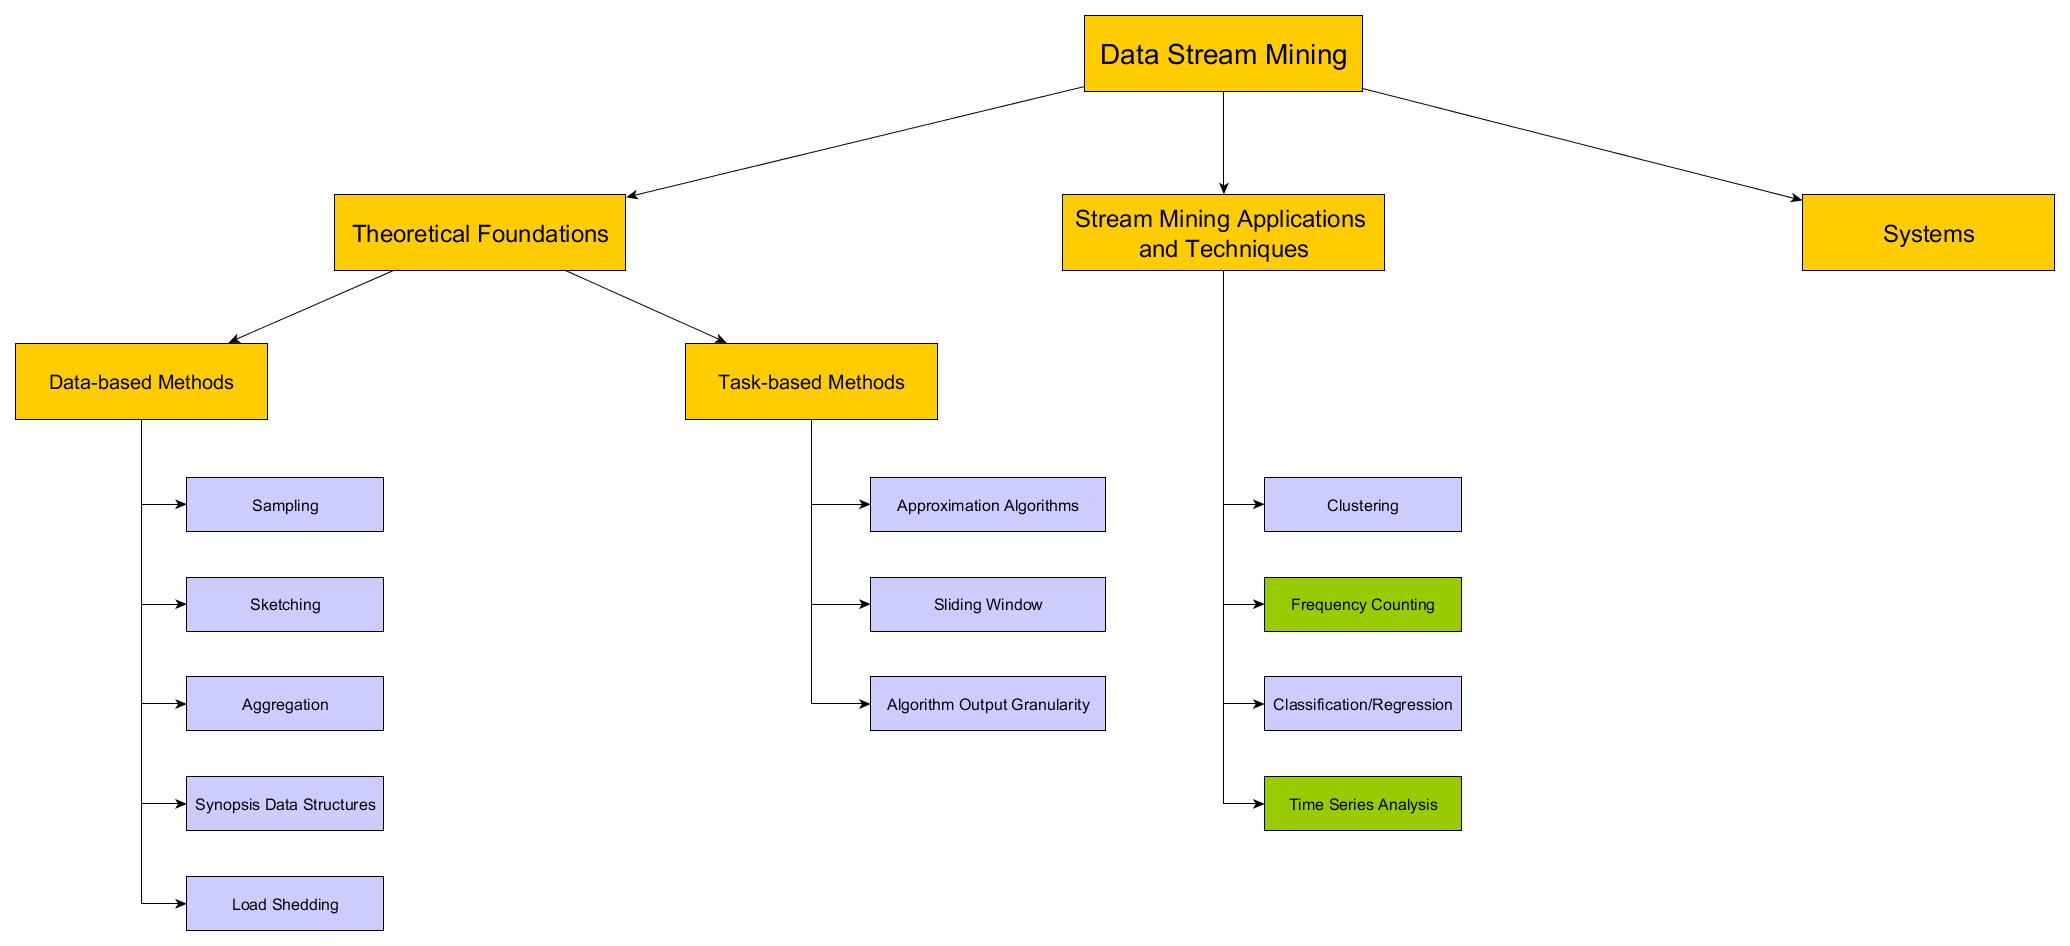
\includegraphics[width=\textwidth]{streamMiningTaxonomy}
	\caption{A taxonomy of the research areas of data stream mining.}
	\label{fig_streamMiningTaxonomy}
\end{figure}

Figure \ref{fig_streamMiningTaxonomy} shows that the state of the art in data stream mining can be roughly divided into three basic parts: Theoretical Foundations, Mining Techniques and Applications as well as Systems. The theoretical foundations deal with general approaches on how to deal with the issues of data streams. Some notable techniques are sampling \cite{manku1999random}, the usage of synposis data structures or approximation algorithms like the lossy counting algorithm \cite{manku2002approximate} as well as the focus on the most recent events by using sliding windows \cite{gama2010knowledge}, which are incrementally updated.\\
The second category contains the actual mining techniques and applications, which are well known from classical data mining. Most relevant to this thesis are the research areas pattern mining algorithms, prediction strategies and time series analysis. Since the latter two research areas are closely linked to each other, they will be discussed in the same subsection.

The last category in the taxonomy is less focused on research issues and conceptual or algorithmic problems but instead lists the existing data stream processing systems (to that date). Since that is less relevant to this thesis we do not mention or describe existing systems but instead refer the interested reader to the original paper by Gaber et. al. \cite{gaber2005mining}. \\
As already mentioned this thesis mainly deals with the subtopics of time series data and pattern mining, which is why these two areas of work will now be inspected more closely in the next subsections.\\

\subsection{Pattern Mining in Data Streams}
\label{subsec_PatternMining}
Arguably the first popular use case of pattern mining in static databases was the mining of frequent itemsets and association rules, which was originally introduced by Agrawal et.al. \cite{agrawal1993mining}. Since then techniques for static databases have evolved. Different approaches, such as candidate generation or pattern growth strategies are nicely summarized in a paper by Han et. al \cite{han2007frequent}. Adapting pattern mining approaches to data streams presents the challenges of limited memory and that the frequency of patterns changes over time. The groundwork for a lot of algorithms was laid by a paper suggesting two approximation algorithms to maintain approximate frequencies: the sticky sampling and the lossy counting algorithm \cite{manku2002approximate}. Originally these algorithms were used to maintain the frequency of items, but the algorithms can be generalized to work for frequent itemsets, too. A slightly different approach was chosen by Gianella et. al. who have developed an algorithm to incrementally maintain approximately frequent itemsets for the most recent time windows using tilted time window frames \cite{giannella2003mining}. Another different approach is to mine the exact set of frequent itemsets, but only maintain the most recently frequent ones \citep{tanbeer2009sliding}. The authors of this paper use a sliding window and tree-restructuring algorithms to achieve this goal. This work is extended by Lee et.al. by focussing on maximal patterns \cite{lee2014sliding}. \\
It is important to keep in mind that mining frequent itemsets is just a subarea of the much more general field of pattern mining. Mining interesting or frequent patterns can be done in many different data representations, such as sequences \cite{mendes2008stream} or graphs. Approaches are often similar, but differ in details. The patterns that will be focused on in this thesis are episodes. To the best of the authors knowledge, there have not yet been any approaches to maintain frequent episodes in data streams. It should be noted that authors of papers concerned with episode mining sometimes use the terms \textit{data stream} and \textit{sequence} interchangeably, since they refer to data streams but then use algorithms that require multiple passes over the data, which is only possible if given static sequences. Since episode mining is a core topic of this thesis, it is dealt with exclusively in section \ref{sec_episodes}.


%As already mentioned many data mining algorithms for data streams make compromises of some sort or employ appoximations. Especially in the area of pattern mining there are quite a few approaches that use approximations or focus on the most recent data. Gianella et. al. have for example developed an algorithm to incrementally maintain approximately frequent itemsets for the most recent time windows using tilted time window frames \cite{giannella2003mining}. Approaches to mine frequent items without tilting the time windows exist as well, such as the sticky sampling or the lossy counting algorithm \cite{manku2002approximate}. These algorithms can be generalized to mine frequent itemsets, too. If this is done however pruning the candidates may become an issue if the main memory is small (the number of candidates to maintain may be too large). \newline
%A paper also related to regression and time series forecasting was published by Papadimitriou et. al. \cite{papadimitriou2003adaptive}. The authors tackle the problem of cyclic time series mining, as well as time series prediction of numerical values in potentially infinite data streams. \newline
%The rise in popularity of mining data streams also pushes research areas like distributed data mining, in which parallelized versions of data mining algorithms are researched. Large data streams and distributed systems often go hand in hand, which creates the need for distributed algorithms. Such solutions have been researched for example for frequent pattern mining \cite{lin2015fast}, association rule mining \cite{ashrafi2004odam}, clustering \cite{januzaj2004dbdc} and classification (in this case a distributed boosting algorithm) \cite{lazarevic2001distributed}. \newline
%A slightly different direction to data stream processing is querying data streams. Some contributing data scientists have thus approached streams in a similar manner as relational databases \cite{motwani2003query}. The authors present their progress at building a general purpose Data Stream Management System (DSMS) prototype, as a pendant to the traditional Database Management Systems (DBMS). They suggest the usage of an extension of SQL as a stream query language to allow for continuous queries and discuss approximation techniques. 


%Of all the fields related to this thesis basic pattern mining is arguably the most well researched and widely used related research area. First to mention are of course the standard pattern mining algorithms for frequent itemsets \cite{han2007frequent}. The authors of this paper nicely summarize different approaches, which either use candidate generation and the apriori-principle or pattern growth strategies. Problematic with the original Apriori-Algorithm is of course that while the apriori-principle helps to prune the candidate generation, its runtime can still be exponential. On top of that it requires multiple passes over the database, which is something that can be impossible given large data streams. These general pattern mining algorithms have of course already been modified or improved for more specific purposes. For example event data logs have been used to build predictive models that search for patterns that predict critical events in the log file \cite{chen2014pattern}. \newline
%A rather large subfield of pattern mining is the field of (business) process mining. This particular domain usually evaluates log-files of (business) applications that log sequences of events. These logs can be mined to satisfy many different information needs, for example clustering \cite{vaarandi2015logcluster} or process models \cite{priyadharshini2016analysis}.
%Another approach in the field of business logs and process mining is outlier and anomaly detection \cite{sureka2015kernel}. The authors use the length of the longest common subsequence between event sequences as a distance measure to find unusual patterns of events. This field of interest is especially interesting since there are a lot of business applications, some of which use legacy software, whose behaviour is at times unclear or error-prone. Mining underlying business models or unusual behavior can help identify errors. \newline
%A subfield of pattern mining that is especially relevant for this thesis is sequential pattern mining. Comprehensive overviews are given by Slimani et al. \cite{slimani2013sequential} as well as Zhao at al. \cite{zhao2003sequential}.



\subsection{Prediction and Time Series Analysis in Data Streams}
\label{subsec_timeSeriesAnalysis}

TODO:


\begin{itemize}
	\item \textbf{Clustering} There are many different approaches that try to apply clustering algorithms to the data stream scenario. Some authors introduce novel methods \cite{aggarwal2003framework} \cite{aggarwal2004framework}, while others modify existing clustering algorithms \cite{guha2000clustering}.
	\item \textbf{Classification and Regression} In Addition to time and memory constraints classification and regression in evolving data streams presents the extra challenges of concept drift, which means that the underlying class distribution may change, which will make the originally built model invalid over time. A commonly used approach to the time and memory constraints are the so-called very fast decision trees \cite{domingos2000mining} which can be built incrementally and require constant time and memory per example.
	\item \textbf{Frequency Counting} Frequency counting is mainly used in conjunction with pattern mining. It is a little unclear why Gaber et. al. decided to name the category frequency counting instead of pattern mining, since all examples that they mention in the frequency counting section of their review count frequencies of items or itemsets, which fit into the category of pattern mining. A reason could be that there exist approaches to counting frequencies that could be generalized to many different pattern mining problems.
	\item \textbf{Pattern Mining} As already mentioned, Gaber et. al. do not explicitly mention pattern mining as a category, however since it is a large field of work and is relevant to this thesis it definately needs to be mentioned. In fact pattern mining in data streams will be looked upon in subsection \ref{subsec_PatternMining} in detail. 
	\item \textbf{Time Series Analysis} Just like pattern mining, time series analysis is especially relevant to this thesis, since predicting (forecasting) future developments based on past data is a large research area in time series analysis. Thus time series analysis in data streams is discussed in detail in subsection \ref{subsec_timeSeriesAnalysis}.
\end{itemize}




Before diving deeper into the topic of time series analysis, it is important to distinguish time series from data streams. Both concepts are similar and also have overlapping research areas. In this thesis we speak of a time series if we refer to a temporally ordered sequence of data points. Usually time series contain numerical values, examples of such data are:

\begin{itemize}
	\item values of a stock market index over a trading day
	\item measurement values sampled from continous readings of a temperature sensor
	\item electrocardiography readings of a human heart
\end{itemize}

Data streams are also ordered sequences of data. The important distinctions between time series and data streams are: 

\begin{itemize}
	\item Data streams continuously have new data points coming in, thus are continuously growing. This does not have to be the case for time series data. A database that records electrocardiography readings of different patients still contains time series data, however these are not data streams, since the readings are finished and no longer updating.
	\item In contrast to time series it is common in data streams to have streams of categorical values or events, whereas values of time series are usually numeric.
\end{itemize}

The combination of both, a time series data stream, is a time series that is constantly updating, for example an electrocardiography reading that is currently taking place, or stock values that are being recorded over a day. In these cases the time series must be processed online. \newline
Most other research areas in data mining such as clustering or classification are rather focussed in their goals (find an appropriate clustering or build an acurate classifier). In contrast to this the research area of time series analysis is more broad, meaning there are a variety of different objectives that can be of interest when analyzing time series. Thus it is helpful to first get an overview over the most common objectives and techniques in a similar way as the taxonomy for data stream mining visualized in figure \ref{fig_streamMiningTaxonomy}. The main source for this subsection is the book by J. Gama \cite{gama2010knowledge}. Figure \ref{fig_timeSeriesInDataStreamsOverview} visualizes the different areas of interest in time series analysis in data streams mentioned by the author.

\begin{figure}[h]
	\centering
  	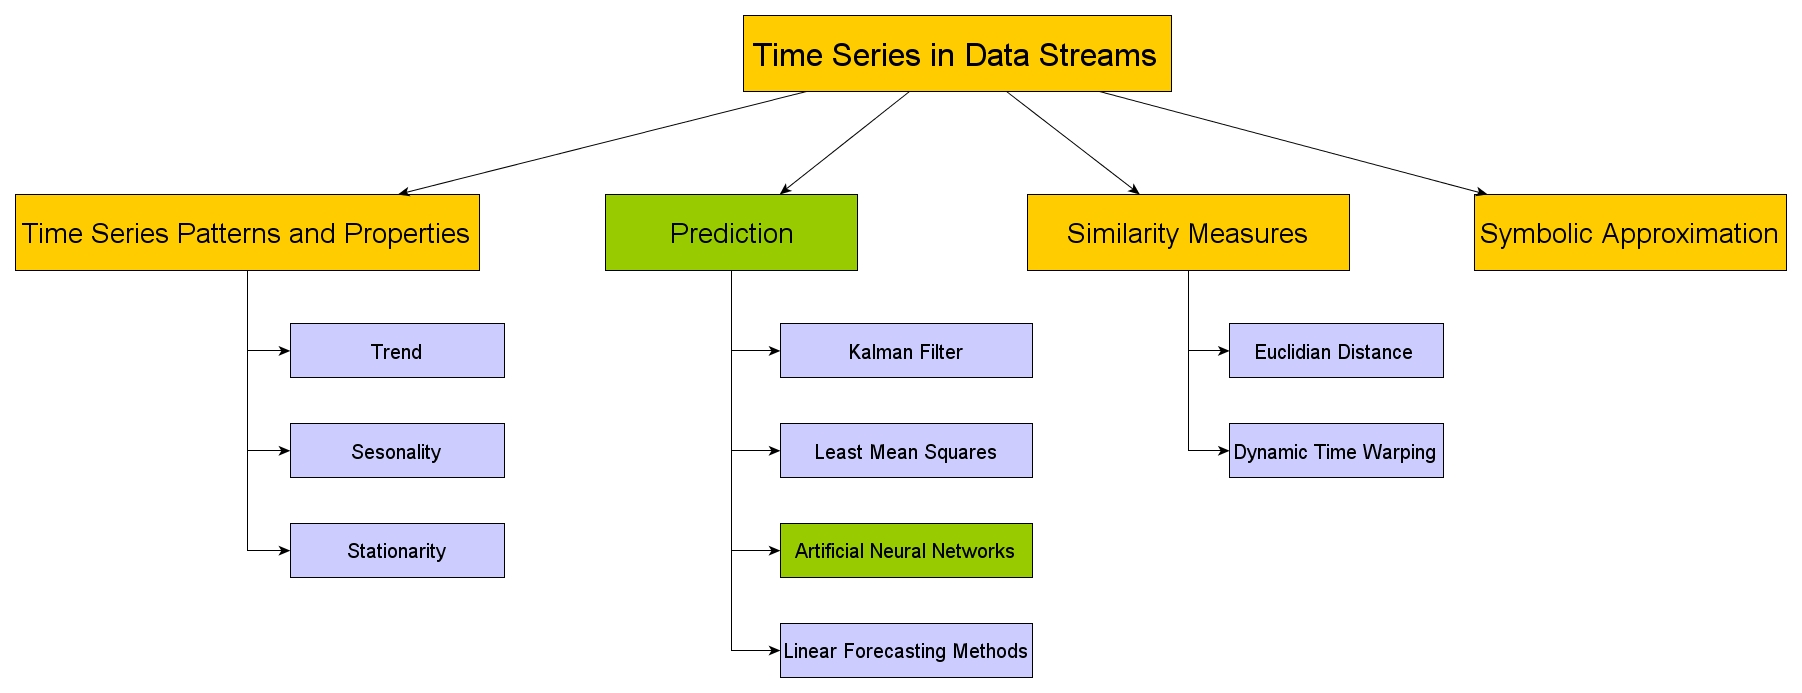
\includegraphics[width=\textwidth]{timeSeriesInDataStreamsOverview}
	\caption{An overview over the different research areas in time series analysis in data streams. The subcategory \textit{"Prediction"} is marked green, since it is of special interest in this thesis and thus will be discussed more extensively than the others.}
	\label{fig_timeSeriesInDataStreamsOverview}
\end{figure}

Note that the research area of time series analysis is large and therefore there are important subareas that are not mentioned by the author. Examples of such research areas are curve fitting, function approximation and time series segmentation. We briefly go over the different areas that are mentioned by J. Gama but are not particularly relevant to this thesis:

\begin{itemize}
	\item \textbf{Time Series Patterns and Properties:} A lot of time series can be categorized according to their behavior and can be said to have certain properties. Among these are for example long term trends, seasonality (cyclic behavior) and stationarity ( mean, variance and autocorrelation are constant).
	\item \textbf{Time Series Similarity Measures:} Similarity of time series has many applications and can for example be used in k-NN classification. There are different similarity measures, which each have their advantages and disadvantages. Two well known examples are the classic euclidean distance and the dynamic time warping algorithm.
	\item \textbf{Symbolic Approximation:} Symbolic Approximation is a technique that aims to discretize time series into a string of arbitrary length. It can be of interest if one wants to apply algorithms that work on strings or categorical data to time series.
\end{itemize}

Obviously, time series prediction (also called forecasting) is a large research area, which is often specialized for individual domains. Therefore, we will give a broad overview here and go into more detail in the next subsection, where we report the state of the art on the prediction of financial time series. \\
Very broadly forecasting methods can be divided into linear and non-linear methods. Linear models are usually simpler, but are at a disadvantage when the underlying model is non-linear \cite{zhang2003time}. Non-linear methods, such as neural networks are more powerful, in fact it has been shown that neural networks can in theory model any non-linear function \cite{abraham2005artificial} \cite{funahashi1989approximate}. However, building and training an actual neural network is a difficult task, since multiple design choices (such as the number of hidden neurons, the activation function and the initial weights) need to be made, which usually requires expert knowledge of both the underlying domain as well as neural networks in general in order to train an appropriate network \cite{abraham2005artificial}. Researchers have also tried to combine both approaches in order to form hybrid methods \cite{zhang2003time}. \newline
Neural networks were originally conceived as batch methods, meaning there were used in an offline scenario with no new data coming in constantly. However adapting them to the stream environment is surprisingly simple in most cases and has been done on multiple occasions \cite{chang2002real} \cite{frank2001time}. In fact, the streaming environment can be beneficial to neural network training, since training a neural network in a static environment usually means making multiple passes over the training data, due to the lack of training data. If done incorrectly this can result in overlearning the training data and thus poor generalization. In the streaming environment however, there is an abundance of data, which means that each example has to be processed only once \cite{gama2010knowledge}. \newline
Predicting or forecasting time series values is normally very domain specific which results in different domains having their own specialized forecasting methods or specific modifications of popular general predictive models. Some of the domains in which time series forecasting is relevant are:

\begin{itemize}
	\item Forecasting price developments in stock markets (see section \ref{sec_stock_market_prediction} for a detailed review of the state of the art)
	\item Forecasting the electricity demands of households \cite{veit2014household}
	\item Forecasting the power output of solar energy plants \cite{inman2013solar}
\end{itemize}


%
%
%\subsection{Classification and Regression}
%\label{subsec_regression}
%
%Classification and regression are the main applications of supervised learning. They are very similar and closely interlinked to each other. Classification aims to assign new, unseen objects to a class based on a model that was created from training data. Class labels are categorical. Regression is similar, but instead of assigning categorical class labels to new data points it is now the goal to generate a numerical (real) value that is close to the actual value. 
%A comprehensive overview over most classification approaches was comprised by Kotsiantis et. al. \cite{kotsiantis2007supervised}. The authors distinguish between different types of classifiers:
%\begin{itemize}
%	\item logical classifiers such as Decision Trees and rule based algorithms
%	\item preceptron based classifiers, such as the single layered perceptron or artificial neural networks
%	\item statistical classifiers, such as naive bayes or bayesian networks
%	\item instance based classifiers, such as k nearest neighbor
%	\item maximum margin classifiers, such as support vector machines
%\end{itemize}
%It is notable that the authors do not mention ensemble learners \cite{dietterich2000ensemble}, which combine several classifiers and classify new examples by letting each classifier vote. Arguably the most notable ensemble learning technique is the random forest \cite{liaw2002classification}.
%It is important to keep in mind that most classification approaches can also be tweaked to do regression, a random forest for instance can either be used to estimate a (binary) class label (classification) or a numerical value (regression).
%Classification and regression have also been attempted by using pattern mining and association rule generation \cite{ma1998integrating}. Instead of mining all association rules the authors focus on finding so called class association rules. An especially relevant application of rule based regression was the usage of classification rules using minimal rule generation for the prediction of equity returns \cite{apte1994predicting}. The authors modify a classification rule generation technique called R-MINI to be able to do regression. They evaluate their approach on historical stock market data from the S\&P 500 data-set (data is aggregated to monthly values). 
%While both of these pieces of work are interesting and extremely relevant to the problem tackled by this thesis it is important to note that they were both done in 1998 and 1994 respectively, so it is expected that the state of the art has changed since then.



%\subsection{Complex Event Processing and Episode Mining}
%\label{subsec_eventProcessing}
%Before talking about the state of the art in complex event processing it is first important to clarify the term \textit{"event"} which is a is very broad term that is used in many different areas of science. Even when restricted to computer science there may be different definitions with subtle differences. As already explained in the introduction this thesis will focus on events as defined by the glossary of the event processing society \cite{luckham2011epts}.
%When talking about processing complex events there is an important difference between two cases:
%
%\begin{itemize}
%	\item The patterns of interest are known before looking at the data. This is called complex event detection.
%	\item There is no prior knowledge about which patterns might be interesting, they need to be discovered while looking at the data. This is called complex event discovery or complex event mining (which basically means that data mining methods need to be employed)
%\end{itemize}
%
%Complex event detection usually revolves around specification and query languages for complex events \cite{eckert2009complex}. Quite a few different specification and query languages have been developed, such as SNOOP \cite{chakravarthy1994snoop} or the SASE event processing language \cite{wu2006high}. \newline
%Discovering interesting complex events of arbitrary structure in data streams is a very challenging task, thus most work focuses on specific types of complex events. A popular example is mining frequent sequences of events (basically complex events that only use the sequence operator) \cite{bettini1998mining} \cite{hasan2015probabilistic}. \newline
%This thesis deals with a more expressive type of complex events: Episodes. Originally episodes were researched without any relation to event processing \cite{mannila1995discovering}. 
%Episodes have roughly been categorized as serial, parrallel or composite and there are different mining methods proposed for each of these \cite{mannila1995discovering} \cite{zhou2010mining}. The connection between episodes and hidden markov models was also explored in a PHD thesis by Laxman \cite{laxman2006discovering}.
%Evaluating episode mining algorithms on real-life datasets is often difficult due to a lack of knowledge about the ground truth. Thus, generation of realistic, synthetic datasets has been looked into as well \cite{zimmermann2012generating}.



\section{Stock Market Forecasting}
\label{sec_stock_market_prediction}
When reviewing the related work for the forecasting of stock markets, it is important to note that in a lot of cases, financial time series are not analyzed in a streaming environment. Authors commonly attempt to forecast daily closing values of stock markets, which means that in this case data velocity is very low (one new data point per day). However many techniques applied in these scenarios can also be applied in more rapidly moving streams. Examples of these are autoregressive models \cite{terasvirta1994specification} or artificial neural networks \cite{gama2010knowledge}. \newline
A good starting point into the prediction of stock market movements is provided by a literature study by Atsalakis et. al. \cite{atsalakis2009surveying}. The authors review more than 100 papers that attempt to predict stocks or stock indices. Figure \ref{fig_financialTimeSeriesPredictionOverview} visualizes some of the different properties and experimental settings of the approaches covered by Atsalakis et. al.

\begin{figure}[h]
	\centering
  	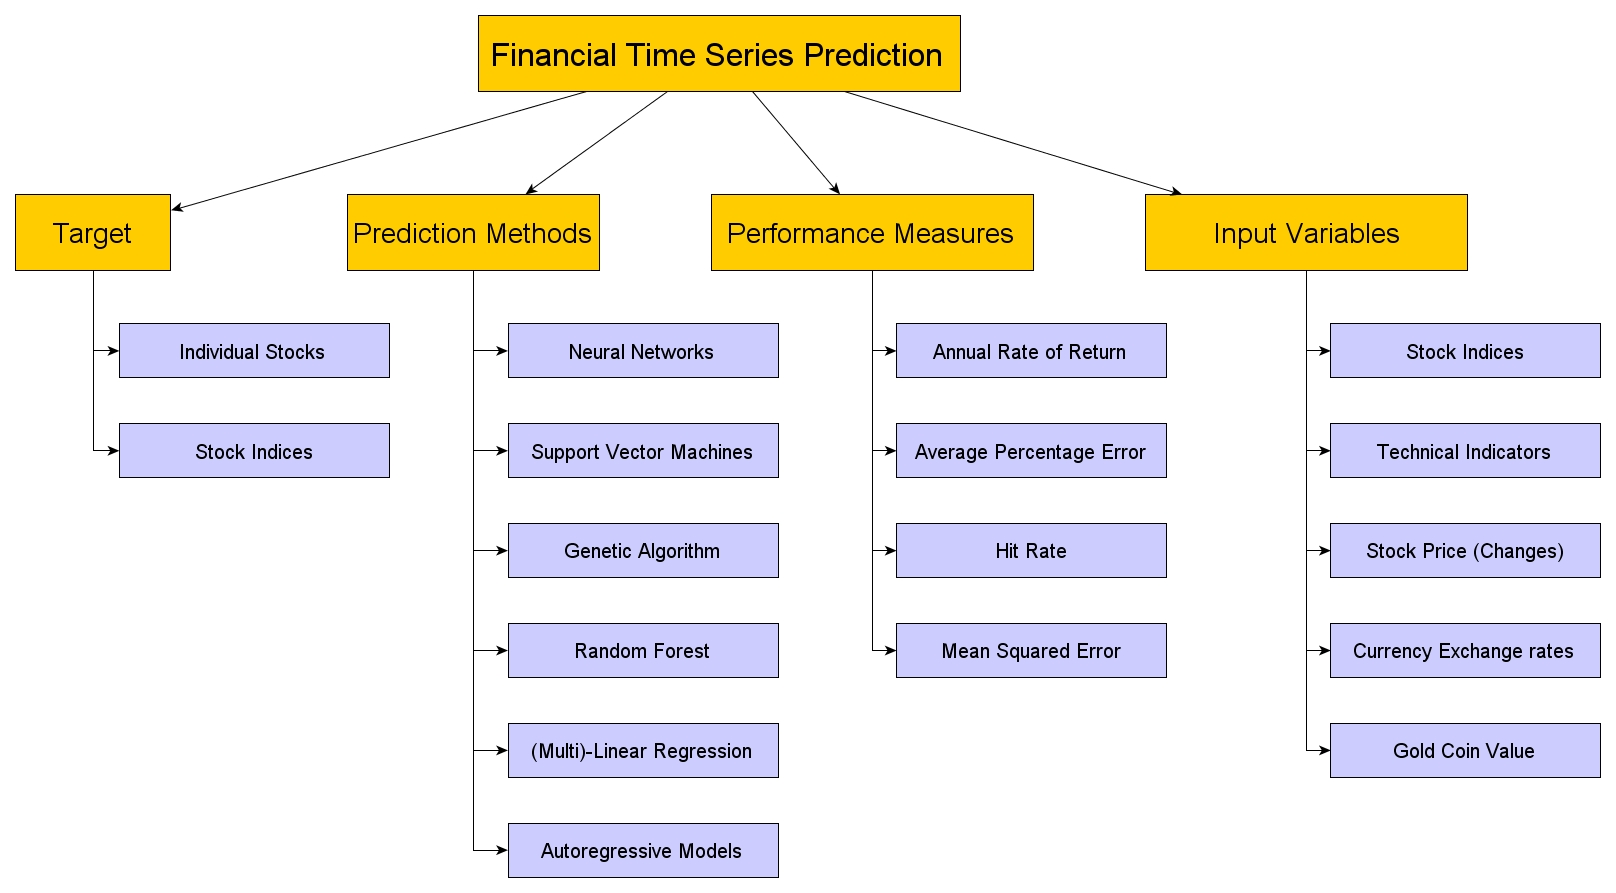
\includegraphics[width=\textwidth]{financialTimeSeriesPredictionOverview}
	\caption{An overview over different properties, experimental settings and approaches to the forecasting of of stock markets}
	\label{fig_financialTimeSeriesPredictionOverview}
\end{figure}

Most of the visualized information in figure \ref{fig_financialTimeSeriesPredictionOverview} was taken from the previously mentioned literature study by Atsalakis et. al. \cite{atsalakis2009surveying}. However  some pieces of work were not covered in that study, for example a comparative study of different models including the otherwise rarely used random forest \cite{kumar2006forecasting}. We briefly review the different properties and categories visualized in figure 
\ref{fig_financialTimeSeriesPredictionOverview}:

\begin{itemize}
	\item \textbf{Target:} The target that is to predict can in theory be any financial index, indicator or price of interst. Many researchers tried to forecast the movement of stock indices \cite{zhang2009stock},\cite{van2001financial}, \cite{kumar2006forecasting} . However, also individual stocks have received attention \cite{mahfoud1996financial}. 
	\item \textbf{Performance Measures:} When building models it is crucial to measure their performance to enable comparison to other models. The number of different performance measures in this case is surprisingly large and diverse. The employed measures range from economic measures, such as the annual rate of return or the Hit-Rate to more technical measures such as the average percentage error or the mean squared error to only name a few. It is impractical to visualize or enumerate all measures that are in use, thus we limit ourselves to the previous examples. For a comprehensive list we refer the reader to the literature study by Atsalakis et. al. \cite{atsalakis2009surveying}.
	\item \textbf{Input Variables:} In real world scenarios this is probably the most important category. No matter which kind of elaborate model is built, if the choice of the input variables is poor, meaning they contain little information, then the model built from those simply can not perform well. This is especially true for financial time series, since those are known to be chaotic and noisy \cite{zhang2009stock}. In fact there are researchers that argue that financial time series follow the principle of random walks which would imply that accurately, meaning better than random, forecasting financial time series based on historical data is impossible. \cite{fama1965behavior}. However there is a considerable amount of papers that suggest otherwise, since accurate prediction results have been achieved by multiple authors based on multiple different forecasting methods (see the literature study by Atsalakis et. al. for examples \cite{atsalakis2009surveying} ). Input variables for stock market prediction are almost always past stock data. Sometimes other financial indicators are used as well. Examples include different stock indices, gold price or currency exchange rates.
	\item \textbf{Prediction Methods:} While figure \ref{fig_financialTimeSeriesPredictionOverview} mentions many different approaches to the forecasting of stock markets, a large majority of the published papers in this area uses some form of neural network. In fact Atsalakis et. al. note that 60\% of the papers they surveyed use feed forward Neural Networks and recurrent networks \cite{atsalakis2009surveying}. 
\end{itemize}

TODO: formulate a nice conclusion


%Similar to regression and classification, but not quite the same is prediction. Prediction (sometimes also called forecasting) introduces a new dimension, which is time. The task in prediction is to build a model that if given data points on a timeline will predict which data point will show up next.
%Due to its dependency on time, prediction plays a large role when mining time series data. Arguably the most popular models for time series prediction are artificial neural networks which are used by multiple authors with differnt variations and application domains \cite{connor1994recurrent} \cite{martinetz1993neural} \cite{frank2001time}. Of particular interest for this thesis are of course prediction approaches that were used in the same domain, namely stock market or financial time series prediction. Naturally this has been looked into. Gestel at. al. used support vector machines to predict the closing values of stock market indices \cite{van2001financial}.% (TODO: Talk/Read more about this paper, the bayesian networks, that are used too) 
%Another, more recent approach used an artificial neural network with an improved learning algorithm (by integrating improved bacterial chemotaxis optimization into the back propagation of the neural network) to successfully predict the Standard’s \& Poor’s 500 index (changes were aggregated to daily values).
%Another different approach is to use grey system models to predict time series \citep{kayacan2010grey}, in this specific case the authors predict the daily foreign currency exchange rate of euro to dollar. A comprehensive comparison of different models for predicting the S\&P CNX NIFTY index was carried out by kumar et. al. \citep{kumar2006forecasting}. The best performing model in their study is the support vector machine, closely followed by a random forest. This is interesting, since random forests have not received as much attention for time series prediction as for example artificial neural networks. Of course no general conclusions can be drawn from the performance of these models for one index. An very detailed overview over a lot of work in the area can be found in the literature study done by Atsalakis et al. \cite{atsalakis2009surveying} although the focus seems to be on papers that use neural networks or support vector machines.
%The attentive reader will have noticed that most of the previously named examples focus on predicting stock indices, a.k.a the general direction of the market. Predicting individual stock values has been looked at less, but there is of source some previous work to be considered. For example mahfoud et. al. compare genetic algorithms to neural networks for the prediction of individual stocks \cite{mahfoud1996financial}.





\section{Episodes}
\label{sec_episodes}
As already mentioned in the introduction, this thesis deals with a specific type of complex events called episodes. Despite being a rather specialized area of research there exists quite a bit of related work that deals with episode mining. What is notable is that there are some discrepancies in terminology. Different authors sometimes use different terms to refer to the same concept or use the same term but with  a different meaning. These discrepancies will be mentioned here and the exact definitions for this paper will be mentioned in chapter \ref{chapter_background}. \\
Before diving into the previous work on episodes it is important to have a rough idea of what kind of patterns episodes are. Thus we provide a short and informal explanation here, whereas section \ref{sec_episodeMiningBackground} will give a much more detailed and formal definition of all concepts revolving around episodes. \\
Most simply put, episode patterns are partially ordered sequences of events. They can be visualized as directed acyclic graphs like the example episode shown in figure \ref{fig_exampleCompositeEpisode}. 

\begin{figure}[h]
	\centering
  	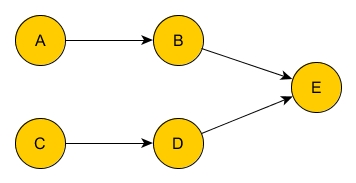
\includegraphics[width=.4\textwidth]{exampleCompositeEpisode}
	\caption{An example episode pattern visualized as a directed acyclic graph. This example pattern specifies that event $A$ and event $C$ may occur in any order, however $A$ must come before $B$ and $C$ must come before $D$, $E$ must occur last.}
	\label{fig_exampleCompositeEpisode}
\end{figure}

Episodes are usually mined from a very large sequence. This distinguishes the concept of episode mining from the concept of sequential pattern mining, which takes place on a sequential database, in which there are many records and each record is a sequence of events \cite{wu2013mining}.
The research concerning episodes can be organized in basic categories as visualized in figure \ref{fig_episodeOverview}.

\begin{figure}[h]
	\centering
  	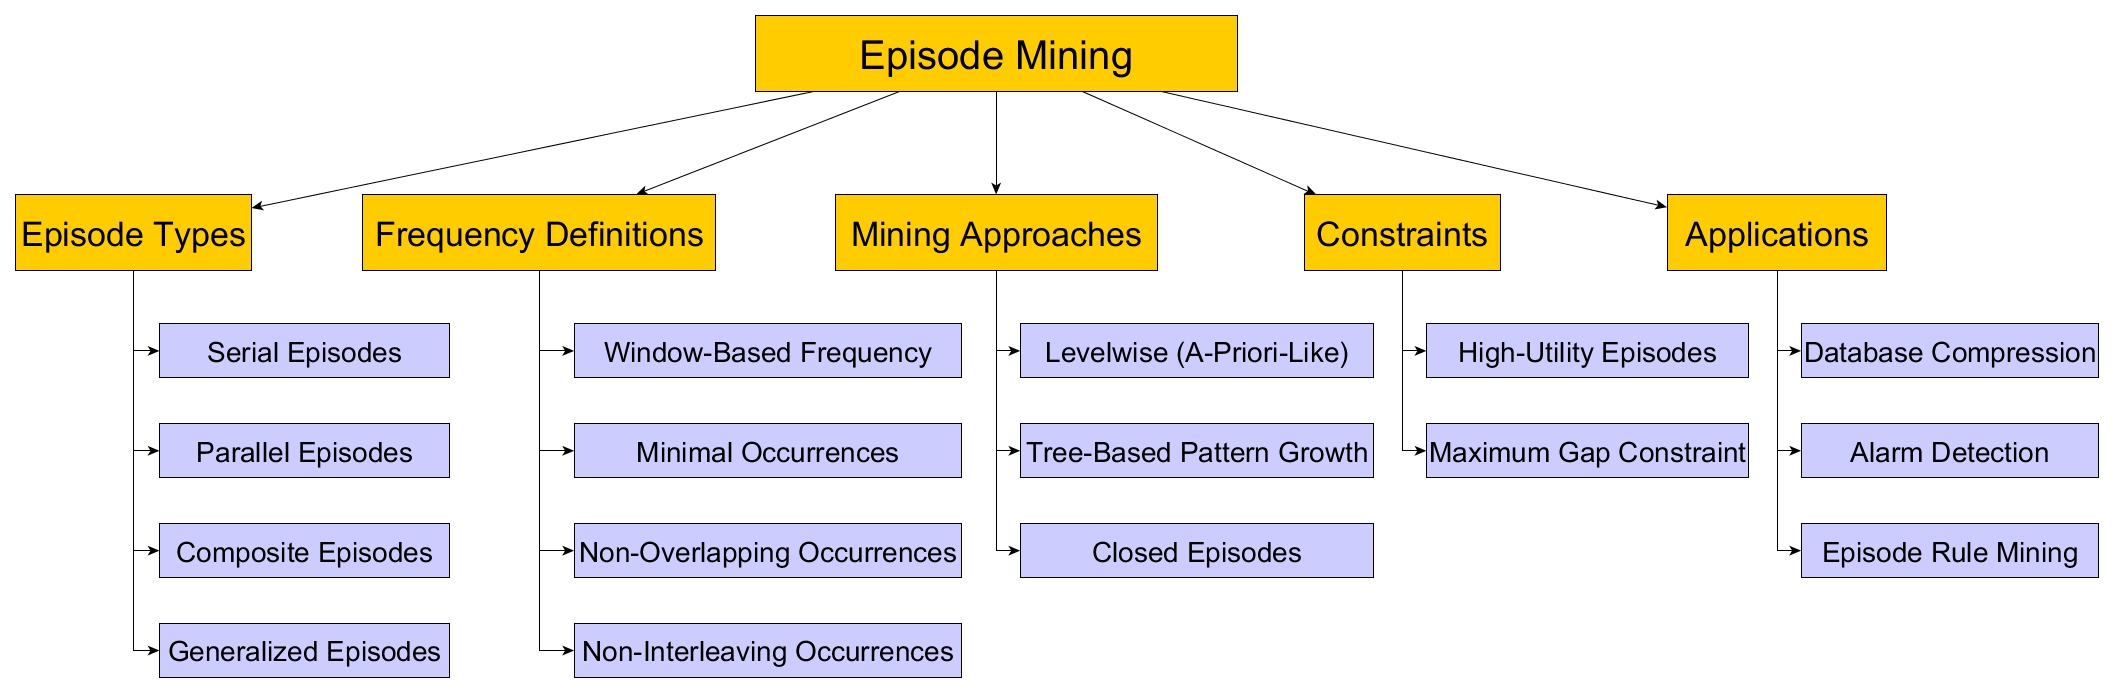
\includegraphics[width=\textwidth]{episodeOverview}
	\caption{A rough categorization of the existing research in episode mining}
	\label{fig_episodeOverview}
\end{figure}

The different types of episodes that have been looked at in the literature are mostly special cases of general episodes. Mannila et. al. introduced the three concepts of serial, parallel and composite episodes \cite{mannila1995discovering}. According to their definitions serial episodes are episodes that have a total ordering (essentially sequences), parallel episodes are episodes without any order (essentially multisets) and composite episodes are episodes that have some order imposed on the events, but do not need to have a total ordering (like serial episodes do). There are however altering definitions of composite episodes in the literature, for example both Bathoorn et. al. \cite{bathoorn2007finding} and Baumgarten et. al. \cite{baumgarten2003tree} deviate from the original definition and redefine composite episodes as sequences of sets. in their works. Section \ref{subsec_basicEpisodeDefinitions} explains the difference between the two definitions in more detail. Extended episodes have been investigated by S. Laxman in his PHD thesis \cite{laxman2006discovering}. The main difference between classic episodes and extended episodes is that classic episodes assume that the basic events are instantaneous, whereas extended episodes can be mined from events that have a duration. It is notable that most work focuses on serial and parallel episodes \cite{mannila1995discovering} \cite{mannila1997discovery} \cite{laxman2006discovering} \cite{laxman2007fast}. Authors have already identified this gap in the research and come up with two different reasons:
\begin{enumerate}
	\item The problem of frequent pattern explosion is already significant for serial and parallel episodes, but still much worse for composite episodes \cite{bathoorn2007finding}.
	\item Detection of composite episodes (checking whether a given composite episode occurs in a sequence) is NP-complete, since 3-SAT can be reduced to this problem \cite{tatti2011mining}.
\end{enumerate}

An exception is a paper by Achar et. al. which introduces an algorithm to mine injective episodes with general partial orders \cite{achar2012discovering}. However the authors still require the episodes to be injective (each event type occurs only once). \\
When mining frequent episodes from sequences, frequency of episodes can be defined in multiple ways. Since the different variants of episode frequency need to be carefully considered in this thesis we do not give a brief overview here but instead devote subsections of chapter \ref{chapter_background} to discuss the different frequency definitions. Specifically subsection \ref{subsec_windowBased} gives a detailed explanation of the window based frequency, whereas subsection \ref{subsec_otherFrequency} provides an overview over the other frequency definitions that have been used in the literature. \\
The different mining approaches for episodes are similar to well known approaches for frequent itemset mining. Since most episode frequency definitions follow the apriori principle, a level-wise approach like in frequent itemset mining \cite{agrawal1993mining} is suggested by many authors \cite{mannila1995discovering} \cite{laxman2006discovering}. As an alternative, tree growth methods have been proposed, in which candidate episodes are represented in a tree data structure that gets grown as the algorithm progresses \cite{baumgarten2003tree}. Since frequent pattern explosion is an issue when mining frequent episodes it is unsurprising that the concept of closed patterns from classical pattern mining \cite{wang2003closet+} has been adapted to episodes \cite{zhou2010mining} \cite{tatti2011mining}. \\
When mining episodes, authors have considered several constraints or specific scenarios. Usually one is interested to mine episodes that are local, meaning the events of the episode are supposed to happen close to each other (time-wise). The maximum duration of an episode can be restrictd in different ways, for example by specifying a window size \cite{mannila1995discovering}, when employing the window-based frequency or by a maximum gap constraint, which restricts the maximum time difference between two events of an episode \cite{meger2004constraint}. Another special scenario that considers external constraints is the mining of high-utility episodes, in which one is not interested in frequent episodes but instead into those episodes that cover events that have a high utility score (which is given externally) \cite{wu2013mining}. \\
Mining episodes from data streams has received attention recently for example by Ao et. al. \cite{ao2015online}, who developed an online mining algorithm for the most recent serial frequent episodes. The similar problem of mining the most recent top-k episodes has also received attenion \cite{patnaik2012efficient}.\\
The applications for episode mining are diverse and some of them are mentioned in the following.

\begin{itemize}
	\item Mannila et. al. (arguably the researchers to make episode mining a popular task) were motivated to mine episodes in order to analyze alarms in telecommunication systems \cite{mannila1997discovery}.
	\item Several authors attempt to describe, summarize or compress databases or large sequences by mining appropriate episodes. Examples of research in this application area include the work by Bathoorn et. al. \cite{bathoorn2007finding} as well as the work by Vreeken et. al. \cite{vreeken2012summarising}.
	\item Episode mining has been used to extract rules from sequences in several different domains, such as geophysics (finding dependencies between earthquakes) \cite{meger2004constraint} or health care (analysis of temoral dependencies between risk factors for atherosclerosis) \cite{meger2004mining}.
	\item Finally, episode mining has been used to build predictive models. Laxman et. al. describe in their paper how they mine serial episodes to learn hidden markov models to predict events in sequences \cite{laxman2008stream}. 
\end{itemize}

\section{Semantic Web}
\label{subsec_semanticWeb}
TODO


%\section*{Subplots}
%I can cite Wall-E (see Fig.~\ref{fig:WallE}) and Minions in despicable me (Fig.~\ref{fig:Minnion}) or I can cite the whole figure as Fig.~\ref{fig:animations}


%\begin{figure}
%  \centering
%  \begin{subfigure}[b]{0.3\textwidth}
%   
\includegraphics[width=\textwidth]{TomandJerry}
%  \caption{Tom and Jerry}
%    \label{fig:TomJerry}   
%  \end{subfigure}             
%  \begin{subfigure}[b]{0.3\textwidth}
%    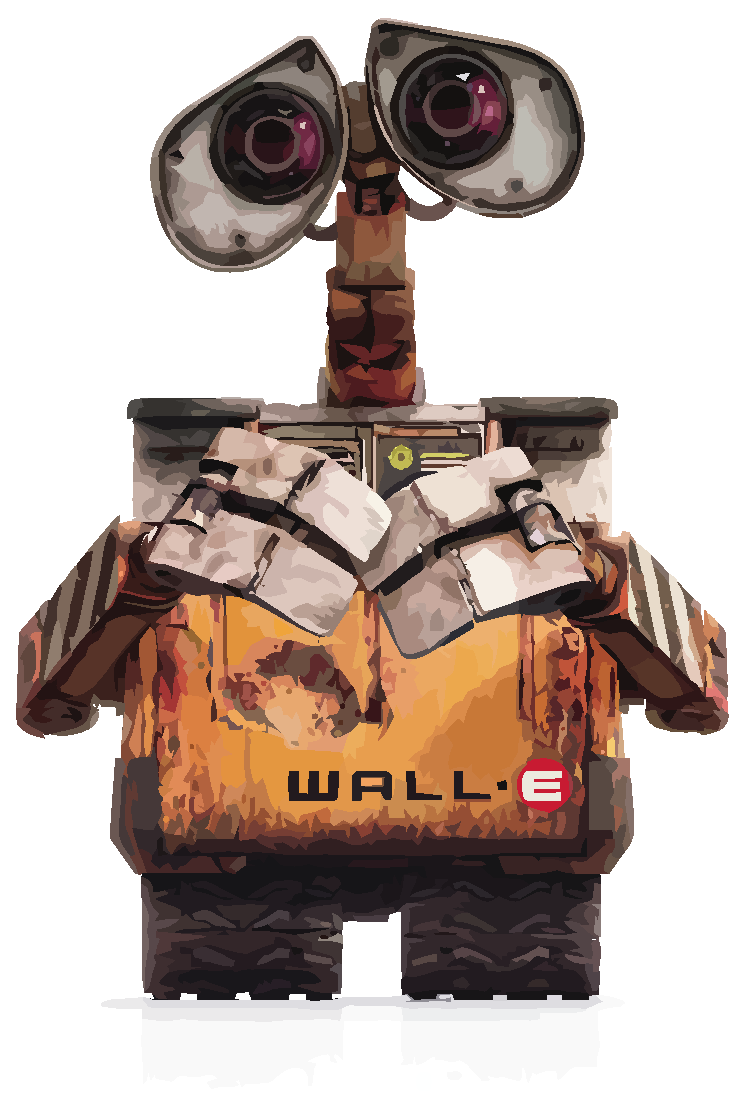
\includegraphics[width=\textwidth]{WallE}
%    \caption{Wall-E}
%    \label{fig:WallE}
%  \end{subfigure}             
%  \begin{subfigure}[b]{0.3\textwidth}
%    
\includegraphics[width=\textwidth]{minion}
%    \caption{Minions}
%    \label{fig:Minnion}
%  \end{subfigure}
%  \caption{Best Animations}
%  \label{fig:animations}
%\end{figure}



\chapter{Episode Mining Background}
\label{chapter_background}

% **************************** Define Graphics Path **************************
\ifpdf
    \graphicspath{{Chapter3/Figs/Raster/}{Chapter3/Figs/PDF/}{Chapter3/Figs/}}
\else
    \graphicspath{{Chapter3/Figs/Vector/}{Chapter3/Figs/}}
\fi

This chapter establishes the terminology and basic formal definitions for this thesis. While episodes were already intuitively defined and talked about in the previous chapters it is important to formally define episodes, since formal definitions are clear and unambiguous. This is important in order to define and explain mining objectives and techniques as well as algorithms that are used in this thesis. 

\section{Basic Definitions}
\label{sec_basicEpisodeDefinitions}
Episodes are complex events whose basic building blocks are simple events. Note that  in order to make use of episodes we require that all simple events have a type and we have a finite, previously known event alphabet, that contains these types, which we refer to as $\Sigma$. We follow up with a formal definition:

\begin{mydef}
\label{def_episode}
\textbf{Episode} An episode (also sometimes called episode pattern or elementary episode) $\alpha$ of length $m$ (also called m-episode) is defined as a triple: $\alpha = (V_\alpha,{\leq}_{\alpha},g_\alpha)$ where $V_\alpha = \{v_1,...,v_m\}$ is a set of nodes, ${\leq}_{\alpha}$ is a partial order over $V_\alpha$ and $g_\alpha : V_\alpha \rightarrow \Sigma$ is a mapping that maps each node of $V_\alpha$ to an event type. \cite{mannila1995discovering}
\end{mydef}

Put more simply an episode is a multiset of event types, whose elements can be, but do not have to be ordered by a relation (${\leq}_{\alpha}$). Another way of putting it is that an episode is essentially a partially ordered sequence of events. Before we look at examples there are a two special types of episodes that need to be mentioned since they have received the most attention in the available literature. These are called serial and parallel episodes:

\begin{mydef}
\textbf{Serial Episode} An episode $\alpha = (V_\alpha,{\leq}_{\alpha},g_\alpha)$ is called a serial episode if ${\leq}_{\alpha}$ is a total order. \cite{mannila1995discovering}
\end{mydef}

\begin{mydef}
\textbf{Parallel Episode} An episode $\alpha = (V_\alpha,{\leq}_{\alpha},g_\alpha)$ is called a parallel episode if ${\leq}_{\alpha} = \emptyset$, in other words if there is no ordering imposed on $V_\alpha$ at all. \cite{mannila1995discovering}
\end{mydef}

Essentially, serial episodes are sequences, while parallel episodes are multisets. Figure \ref{fig_exampleEpisodes} visualizes example episodes in the same way that we have visualized episodes in earlier chapters, namely as directed acyclic graphs (DAG).

\begin{figure}[h]
	\centering
  	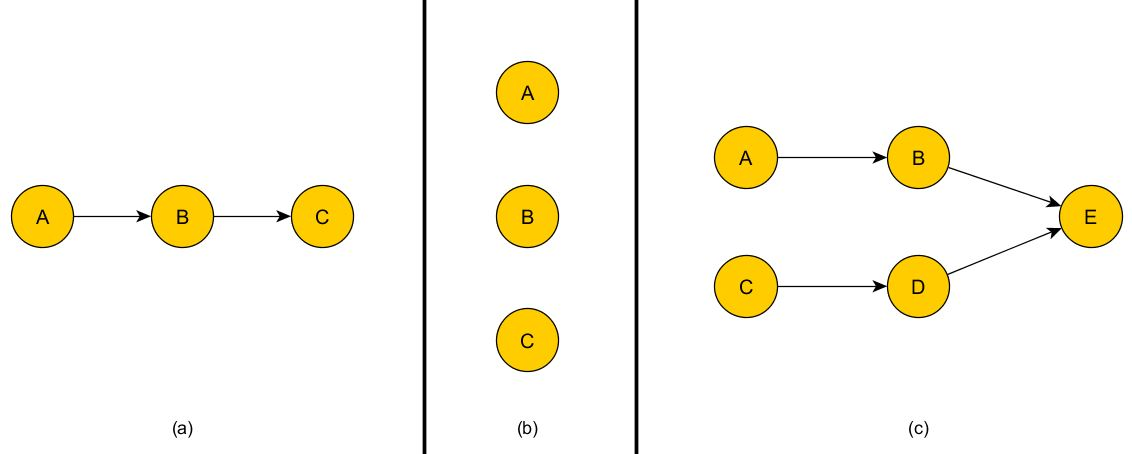
\includegraphics[width=\textwidth]{exampleEpisodes}
	\caption{An example of different episodes: (a) - a serial episode, (b) - a parallel episode, (c) - an elementary (composite) episode}
	\label{fig_exampleEpisodes}
\end{figure}

%\begin{figure}[H]
%\centering
%\begin{tabular}{c|c|c}
%\begin{subfigure}{.3\textwidth}
%  \centering
%  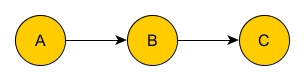
\includegraphics[width=\linewidth]{exampleSerialEpisode}
%  \caption{A serial episode}
%  \label{fig:sub1}
%\end{subfigure}%
%&
%\begin{subfigure}{.3\textwidth}
%  \centering
%  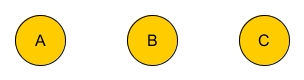
\includegraphics[width=\linewidth]{exampleParallelEpisode}
%  \caption{A parallel episode}
%  \label{fig:sub2}
%\end{subfigure}
%&
%\begin{subfigure}{.3\textwidth}
%  \centering
%  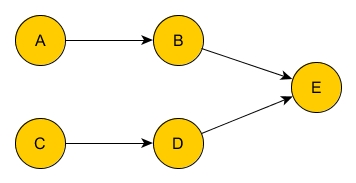
\includegraphics[width=\linewidth]{exampleCompositeEpisode}
%  \caption{An elementary (composite) episode}
%  \label{fig:sub3}
%\end{subfigure}
%\end{tabular}
%\caption{Different example episodes visualized as directed acyclic graphs}
%\label{fig_exampleEpisodes}
%
%\end{figure}

In fact each episode can be formally transformed to a DAG using the following simple procedure: Given an Episode $\alpha = (V_\alpha,{\leq}_{\alpha},g_\alpha)$, create the corresponding DAG $G = (V,E)$ by executing the following:

\begin{enumerate}
	\item For each $v \in V_\alpha$ add $v$ to $V$ and label $v$ with $g_\alpha (v)$
	\item For each pair $v,w \in V_\alpha$ where $v \, {\leq}_{\alpha} \, w $ add edge $(v,w)$ to $E$
\end{enumerate}

The original paper by Manilla et.al. \cite{mannila1995discovering} also introduces the notion of composite episodes. We repeat the definition here:

\begin{mydef}
\label{def_compositeEpisodes}
\textbf{Composite Episode} An episode $\alpha = (V_\alpha,{\leq}_{\alpha},g_\alpha)$ is called a composite episode if $g_\alpha : V_\alpha \rightarrow \Sigma \cup C^*$, where $C^*$ is the set of all composite episodes. \cite{mannila1995discovering}
\end{mydef}

This recursive definition of composite episodes may be confusing at first, since it is formulated very compactly. A slightly more clear way to look at it is the following:\\
A composite episode is either:
\begin{itemize}
	\item A single event (An elementary episode of length 1).
	\item A serial composition of two composite episodes
	\item A parallel composition of two composite episodes
\end{itemize}

This definition has the advantage that any elementary episode can be represented as a composite episode which is exclusively a serial or parallel composition of serial, parallel or composite subepisodes (see definition \ref{def_subEpisode}). Note that composite episodes are not more expressive than elementary episodes as defined in definition \ref{def_episode}, it is just a recursive way of defining episodes. \\
Interestingly, there are other parts of the related work that use the term \textit{composite episodes} but deviate from definition \ref{def_compositeEpisodes}. For example Baathorn et. al. propose a method for finding composite episodes \cite{bathoorn2007finding}. However they define composite episodes as a sequence of parallel episodes, which is more restrictive than the original definition. Also Baumgarten et. al. use this definition \cite{baumgarten2003tree} when they present an approach to mine descriptive composite episodes. Note that not all elementary episodes can be represented as sequences of parallel episode. A simple example shown in figure \ref{fig_notSequenceOfSet} illustrates this.

\begin{figure}[h]
	\centering
  	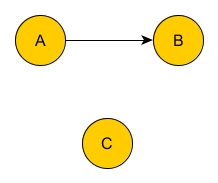
\includegraphics[width=0.3\textwidth]{notSequenceOfSet}
	\caption{An elementary episode that can not be represented as a sequence of parallel episodes}
	\label{fig_notSequenceOfSet}
\end{figure}

If the presented episode were to be represented as a sequence of parallel episodes obviously $A$ and $B$ would have to be in different parallel episodes in order to fulfill the requirement that $B$ must be after $C$. After that the problem is that it is impossible to assign $C$ to any of those sets. If it gets assigned to the same parallel episode set as $A$ then this would prohibit $A$ and $B$ occurring first followed by $C$, which is allowed in the original definition. Likewise if $C$ gets assigned to the same parallel episode as $B$ then that eliminates the possibility of $C$ occurring before $A$ and $B$, which once again was allowed in the elementary episode. In this thesis we will stick to the original definition as presented in definition \ref{def_compositeEpisodes}. \newline
If we want to quickly denote simple episodes formally without drawing a DAG, we will use $\rightarrow$ as the sequence (ordering) operator. To show that there is no order specified between two nodes we use $\|$ as the parallel operator. For example $(A \, \| \, B ) \rightarrow C$ denotes a composite episode of length 3, which specifies that it does not matter in which order $A$ or $B$ occur, but $C$ must occur after both $A$ and $B$. If we want to discuss more complex episodes we will visualize them graphically like in the previous figures. \newline 
In algorithms we use the following notation to access episodes:

\begin{itemize}
	\item for all episodes $\alpha = (V_\alpha,{\leq}_{\alpha},g_\alpha)$ we define $|\alpha | = |V_\alpha|$ as the length of the episode.
	\item for serial episodes we define $\alpha [i]$ as the event type of the i-th node of $\alpha$ with respect to the total ordering imposed on $\alpha$ by ${\leq}_{\alpha}$. In other words $\alpha [i]$ is the i-th element of the sequence of event types, defined by the serial episode $\alpha$.
	\item for parallel episodes $\alpha$ we say that $E \in \alpha$ if there is at least one $v \in V_\alpha$, so that $g_\alpha(v) = E$. In this context we define $count(\alpha,E)= \{v \in V_\alpha \mid g_alpha(v) = E\}$, meaning $count(\alpha,E)$ is the number of nodes in the parallel episode $\alpha$ that have type $E$.
\end{itemize}

The notion of sub- and superpatterns, which is very important for most pattern mining applications also applies to episodes, as shown in the next definition.

\begin{mydef}
\label{def_subEpisode}
\textbf{Subepisode} An episode $\beta = (V_\beta,{\leq}_{\beta},g_\beta)$ is said to be a subepisode of episode $\alpha = (V_\alpha,{\leq}_{\alpha},g_\alpha)$ if all of the following conditions hold:
\begin{enumerate}
	\item The nodes of $\beta$ are a subset of the nodes of $\alpha$: \\
	$V_\beta \subseteq V_\alpha$
	\item All nodes of $\beta$ are assigned to the same event type as their corresponding nodes in $\alpha$:\\
	 $\forall v \in V_\beta \; : \; g_{\beta}(v) = g_\alpha (v) $
	\item The ordering in $\alpha$ is at least as strict as the ordering in $\beta$:\\
	$\forall v,w \in V_\beta \, , v \, {\leq}_{\beta} \, w \; : \; v \, {\leq}_{\alpha} \, w$
\end{enumerate}
In this context we also refer to $\alpha$ as the superepisode of $\beta$. \cite{mannila1995discovering,laxman2007fast}.
\end{mydef}

It is important to note that in the original definition of sub- and superepisodes by Mannila et. al. \cite{mannila1995discovering}, the first property of the above definition was actually defined as $V_\beta \subset V_\alpha$, which implies that subepisodes would always have to consist of at least one less node than their superepisodes. This definition was changed by Laxman et. al. \cite{laxman2007fast} to allow set equality as well. The implications of this change are that parallel episodes like $A \| B$ are now subepisodes of their serial counterparts of the same length $A \rightarrow B$. In this thesis we stick to the definition that allows set equality between super- and subepisodes. In both cases however subepisodes may relax the ordering specified in their superepisodes. For example if given the serial episode $\alpha =( A \rightarrow B \rightarrow C )$, not only $A \rightarrow B$ is a subepisode of $\alpha$ but also $A \| B$. \\
So far we have talked a lot about episode patterns but we have not yet talked about the detection such episodes in data. It is helpful to think of the episode patterns we have defined above as templates for concrete occurrences. In order to define what we mean by an episode occurrence, we first need to formally introduce the notion of an event sequence.

\begin{mydef}
\label{def_eventSequence}
\textbf{Event sequence} An event sequence is defined as an ordered list of tuples $S = [ (T_1,t_1),..., (T_n,t_n) ] $ where $T_i \in \Sigma$ is the event type of the i-th event and $t_i \in \mathbb{N}^+$ is the timestamp of the i-th event. The sequence is ordered according to the timestamps, which means that $\forall i,j \in {1,...,n} \; i<j \implies t_i \leq t_j$. \cite{mannila1997discovery} %TODO: talk about time equality
\end{mydef}

Note that it is allowed for two or more consecutive elements in a sequence to have the same timestamp. This is necessary in order to allow for multiple events to occur at the same time. The ordering of events with the same timestamp is not further specified and irrelevant in most cases. Another way to define such sequences is to define them as sequences of event sets in which consecutive event sets must all have different timestamps and events that occur simultaneously are part of the same set \cite{bathoorn2007finding}. Definitions from other authors explicitly prohibit two events happening at the same time \cite{baumgarten2003tree}. Which definition is appropriate depends on the context, for this thesis we will stick with definition \ref{def_eventSequence}. \\
Given the notion of an event sequence we can now define episode occurrences:

\begin{mydef}
\label{def_episodeOccurrence}
\textbf{Episode Occurrence} An event episode $\alpha = (V_\alpha,{\leq}_{\alpha},g_\alpha)$ is said to occur in a sequence $S$ if events of the types that the nodes in $V_\alpha$ are mapped to by $g_\alpha$, occur in $S$ in the same order that they occur in the episode. More formally if we are given a sequence of events $S=[(T_1,t_1),...,(T_n,t_n)]$ we can define an occurrence of $\alpha$ as an injective Map $h:V_\alpha \rightarrow \{1,...,n\}$, where $g_\alpha (v) = T_{h(v)}$ and $\forall \, v,w \in V\alpha : v \;{\leq}_{E}\; w \implies t_{h(v)} \le t_{h(w)}$ holds. \cite{mannila1995discovering}
\end{mydef}

An episode pattern in itself does not specify any time span in which the events of the episode must occur, however if given an episode occurrence we can define the duration of that occurrence. Durations of episode occurrences become relevant in practical applications, when we want to forbid episode occurrences that range over a time period that is too large. 

\begin{mydef}
\label{def_episodeOccurrence}
\textbf{Episode Occurrence Duration} The duration of an occurrence is defined as the difference between the timestamps of the last and first event that the episode nodes are mapped to. More formally if given an episode $\alpha$, a sequence $S=[(T_1,t_1),...,(T_n,t_n)]$ and an occurrence $h:V_\alpha \rightarrow \{1,...,n\}$ the episode duration is defined as $t_{last} - t_{first}+1$, where $last = max( \{h(v)| v \in V_\alpha \}$ and $first = min( \{h(v)| v \in V_\alpha \}$.
\end{mydef}

An example of an episode pattern, a sequence and two occurrences is visualized in figure \ref{fig_occurrenceExample}.

\begin{figure}[h]
	\centering
  	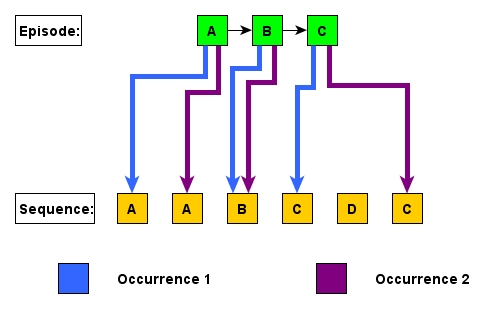
\includegraphics[width=\textwidth]{occurrenceExample}
	\caption{A visualization of the concept of episode occurrences in an event sequence. The episode pattern is drawn in green, the sequence in yellow. An occurrence is defined as a mapping from the nodes of the pattern to events in the sequence (see definition \ref{def_episodeOccurrence}). Thus the occurrences are visualized as arrows of different colors (blue and purple). }
	\label{fig_occurrenceExample}
\end{figure}


\section{Episode Discovery and general Mining Algorithm}
\label{sec_episodeDiscovery}
When discovering episodes in a sequence one is usually interested in those episodes that occur frequently, meaning more often than a user defined threshold. This is similar to all the different kinds of pattern mining algorithms, such as the apriori algorithm for finding frequent itemsets \cite{agrawal1994fast}. A general algorithm for mining the episodes occurring frequently in a sequence is given in algorithm \ref{alg_generalEpisodeMining}. The algorithm is very alike the basic apriori algorithms, since it uses a level-wise, breadth first search by first identifying all frequent episodes of a certain length $i$ and then uses these frequent episodes to generate candidates (possibly frequent episodes) of length $i+1$. In order for this to be correct, episode frequency must follow the apriori principle \cite{agrawal1994fast}, which formally means that if an episode is frequent, all its subepisodes must be frequent as well. Intuitively one would assume that this is always true for episodes but strictly speaking this depends on the definition of episode frequency. However, any frequency definition of episodes that does not satisfy the apriori principle would be highly questionable to say the least, since this would eliminate the possibility of an efficient candidate generation that prunes those episodes which have infrequent subepisodes. To the best of our knowledge all frequency definitions proposed in the literature satisfy the apriori principle.\newline

\begin{algorithm}[H]
  \caption{General mining algorithm for frequent episodes
    \label{alg_generalEpisodeMining}}
  \begin{algorithmic}[1]
    \Statex
    \Function{EpisodeMining}{}
      \Let{$C_i$}{Episodes of Length 1} 
      \Let{$freq$}{$\emptyset$}
      \Let{$i$}{$1$}
      \While{$C_i \neq \emptyset$}
      	\State Count frequencies of each Episode $E \in C_i$
        \Let{$L_i$}{ $\{ E \mid E \in C_i \land C_i \; is\; frequent\}$}
        \Let{$freq$}{$freq \cup L_i$}
        \Let{$C_{i+1}$}{Generate Episode Candidates of length $i+1$ from $L_i$}
        \Let{$i$}{$i+1$}
      \EndWhile
      \State \Return{$freq$}
    \EndFunction
  \end{algorithmic}
\end{algorithm}


In summary, the general mining algorithm for frequent episodes requires:

\begin{itemize}
	\item A definition of episode frequency, that does not violate the apriori principle
	\item An algorithm for counting episode frequency (of concrete candidates) according to this definition
	\item An algorithm to generate candidate episodes
\end{itemize}

It may be a bit confusing that we need a definition of episode frequency for such a mining algorithm. Since we have already defined what an occurrence of an episode looks like it would seem that counting all occurrences of an episode would yield its frequency. While this is a possible definition of frequency, it is important to note that finding all occurrences of an episode within a sequence is neither practical nor useful. An example will demonstrate the problem with this. Consider the simple serial episode $A \rightarrow B$ and a sequence of length $2\cdot n$ which repeats the subsequence $(A,B)$ $n$ times. One quickly realizes that the number of episode occurrences is very large due to the possibility of overlapping episode occurrences. In this particular case there are already $ \frac{n \cdot (n+1)}{2}$ possible occurrences. This number swiftly increases with the length of the episode pattern, since it introduces more potential overlappings. Naturally the number of possible parallel and composite episode occurrences is even larger, since they are less restrictive in the order of the events. Additionally, such a frequency definition would violate the apriori principle, since subepisodes can have less occurrences than their superepisodes. Consider the example sequence $[A,B,C,A,B,C]$ (timestamp values are left out). In this sequence there are 3 distinct occurences for the episode $A \rightarrow B$ and four distinct occurrences for its superepisode $A \rightarrow B \rightarrow C$. These detrimental effects of this naive frequency definition are nicely summarized by Laxman et. al. in a paper presenting the non-overlapped frequency definition \cite{laxman2007fast}. \newline
This leads to various frequency definitions of episodes in the literature, which will be dealt with in subsections \ref{subsec_windowBased} and \ref{subsec_otherFrequency}. Each frequency definition comes with its own frequency counting algorithm. The procedure for generating candidates is independent of the frequency definition and is presented in \ref{subsec_candidateGen}. \newline
%The first two definitions, which we will refer to as window based frequency and minimal occurance based frequency, are mentioned by Zimmermann, when he presents his method for synthetic episode generation \cite{zimmermann2012generating}, but were originally conceived in (TODO: include original sources). We refer to the third definition as the non-overlapping occurrence based Frequency which was suggested by Laxman et al. \cite{laxman2007fast}.


\section{Window based frequency}
\label{sec_windowBased}
To the best of our knowledge the window based frequency was the first frequency definition for episodes to gain general popularity. It was conceived by Mannila et. al. \cite{mannila1995discovering}, although the frequency counting algorithms were only mentioned in text form. The same authors  specified the algorithms in a later paper \cite{mannila1997discovery}, which acts as the primary source for the overview given in this subsection. In order to define the window based frequency we first need the notion of a time window: 

\begin{mydef}
\label{def_timeWindow}
\textbf{Time Window} Given a sequence of events $S$ we define the Time Window $W(S,q,r)$ with $q,r \in \mathbb{N}^+$ and $q < r$ as the ordered subsequence of $S$ that includes all events of the annotated event stream $S$ that have a timestamp $t$ where $q \leq t\leq r$. We call $w = r-q+1$ the duration of Window $W$. We denote the size of the window, meaning the number of events in it as $|W|$.
\end{mydef}

An example of how windows of a fixed duration are located in a sequence of events is presented in figure \ref{fig_windowBasedFrequency}.

\begin{figure}[h]
	\centering
  	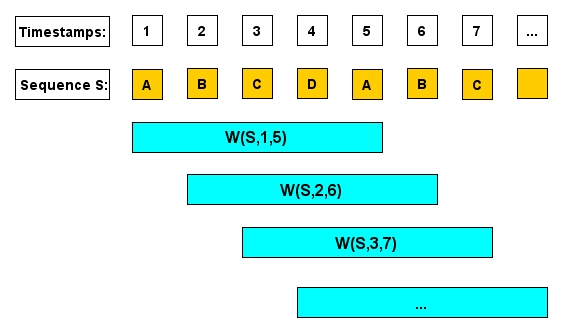
\includegraphics[width=\textwidth]{windowBasedFrequency}
	\caption{Different time windows of duration 5 in an event sequence.}
	\label{fig_windowBasedFrequency}
\end{figure}


\begin{mydef}
\label{def_windowBasedFrequency}
\textbf{Episode Frequency - Window based Definition} Given a sequence of events $S$, a fixed window duration of $w$ and an episode $\alpha$, we define the window based frequency $w\_freq(\alpha )$ as the number of windows $W$ with duration $w$ of $S$ in which $\alpha$ occurs: $w\_freq(\alpha ) = |\,\{W(S,q,r) \mid r-q+1 = w \land \alpha \;occurs\; in\; W \}\,|$. %TODO: incorporate sequence bounds and number of windows
\end{mydef}


For example given the sequence visualized in figure \ref{fig_windowBasedFrequency} $A \rightarrow B \rightarrow C$ occurs in windows $W(S,1,5)$ and $W(S,3,7)$. \newline 
This definition can be confusing at first since it is intended that episode occurrences that are comprised of the exact same events count just as many times as there are windows in which the events appear. In the previously mentioned example, we can find the episode $C \rightarrow D$ in the consecutive windows $W(S,1,5)$, $W(S,2,6)$ and $W(S,3,7)$, which means we will get a frequency of $3$ just for the two events $(3,C)$ and $(4,D)$. This effect obviously increases with the window size. Note that for each episode $\alpha$ we only count one occurrence per window $W$, no matter how many occurrences of $\alpha$ there are in $W$.\newline
When determining the window based frequency the naive approach would be to check each window of the sequence separately. Since the windows are adjacent there is a better approach, which makes it possible to only iterate over the sequence once and determine the window based frequency for each candidate episode. Most papers focus purely on parallel and serial episodes and do not give an algorithm for composite episodes. The algorithms to determine the window based frequency of serial and parallel episodes can be looked up in the appendix \ref{app_freqCounting}.
There is a notable absence of frequency counting algorithms for elementary (composite) episodes in literature. Mannila et. al. claim that each composite episode can be broken down into partial episodes, which are serial and/or parallel \cite{mannila1997discovery}. However they neither specify an algorithm for breaking down composite episodes into purely serial and parallel parts, nor do they specify a frequency counting algorithm for composite episodes. Subsequent research, such as alternate frequency definitions and counting algorithms has also mainly focused on parallel and serial episodes. If composite episodes have been studied they were usually studied in the above mentioned, more restrictive form of sequences of parallel episodes. \newline

\section{Other frequency definitions}
\label{sec_otherFrequency}

In this subsection we briefly present alternative frequency definitions without specifying counting algorithms. For the exact algorithms we refer the reader to the respective papers. \newline
Most alternative definitions tried to move away from the ideas of fixed windows and tried to improve the performance of the counting algorithms. \\
\\
\textbf{Minimal Occurrence Based Frequency Definition} \newline
The first alternate definition does uses the concept of minimal occurrences:

\begin{mydef}
\textbf{Minimal Occurrence} An event episode $\alpha$ is said to occur minimally in a window $W(S,q,r)$ if $\alpha$ occurs in $W$ and there is no subwindow of $W$ in which $\alpha$ also occurs. %(TODO: define subwindow)
\end{mydef}

\begin{mydef}
\label{def_minimalOccuranceFrequency}
\textbf{Episode Frequency - Minimal Occurrence based Definition} Given a sequence of events $S$ and an Episode $\alpha$, we define the minimal occurrence based frequency $mo\_freq(\alpha )$ as the number of minimal occurrences of $\alpha$ in $S$. TODO: find and cite the original source
\end{mydef}

The second alternative definition introduces the concept of non-overlapping occurrences:

\begin{mydef}
\textbf{Non-Overlapping Occurrences} Given a m-Episode $\alpha = (V_\alpha,{\leq}_{\alpha},g_\alpha)$ where $V_\alpha = \{v_1,...,v_m\}$, two occurrences if all timestamps of one of the occurrences are bigger than all the timestamps of the other occurrence. Formally two occurrences $h_1$ and $h_2$ of $\alpha$ are non-overlapped if either:
\begin{itemize}
	\item $\forall \, v_j \in V_\alpha : h_2(v_1)>h_1(v_j)$ or 
	\item $\forall \, v_j \in V_\alpha : h_1(v_1)>h_2(v_j)$
\end{itemize}
A set of occurrences is non-overlapping if every pair of occurrences in it is non-overlapped \cite{laxman2007fast}.
\end{mydef}

An example scenario visualizing overlapping and non-overlapping occurrences is visualized in figure \ref{fig_nonOverlappingExample}.


\begin{figure}[h]
	\centering
  	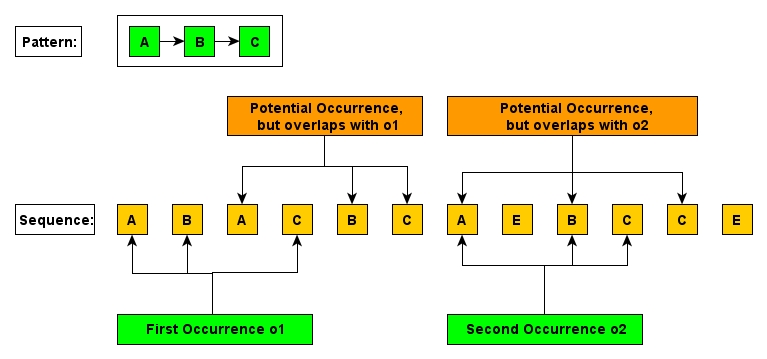
\includegraphics[width=\textwidth]{nonOverlappingExample}
	\caption{An example sequence that shows how occurrences of episode patterns can overlap. Two non-overlapping occurrences are colored in green, whereas the orange occurrences would overlap with one of the green occurrences.}
	\label{fig_nonOverlappingExample}
\end{figure}

This leads to the Definition:

\begin{mydef}
\label{def_nonOverlappingFrequency}
\textbf{Episode Frequency - Non-Overlapping Occurrences based Definition} Given a seqeunce of events $S$ and an Episode $\alpha$, we define the non-overlapping occurrence based frequency $noo\_freq(\alpha )$ as cardinality of the largest set of non-overlapped occurrences of $\alpha$ in $S$ \cite{laxman2007fast}.
\end{mydef}


When looking at these definitions in comparison to the window based frequency definition it is not clear whether any of these is always superior to or more useful than the other since they have different properties. We mention them briefly:

\begin{itemize}
	\item As already mentioned the window based frequency counts an episode occurrence that is comprised of the same events in multiple windows. This might especially distort the count if the window duration is high and the events in the episode happen with minimal delay between them.
	\item The minimal occurrence based definition of frequency does not suffer from the problem of the previous point
	\item The window based definition has the advantage that it already incorporates a fixed duration during which episodes may occur, meaning there can not be episodes that stretch over a time period larger than the fixed window duration $w$. This might be beneficial for potential algorithms, since it reduces the search space for episodes. On top of that it is also closer to reality, since in many domains episodes happen within a small time window.
	\item The non-overlapping occurrence based frequency offers the fastest counting algorithm of all three definitions. However when incorporating expiry times for serial episodes it looses this advantage. Additionally previous literature has not yet identified an efficient algorithm to count non-overlapped occurrences of parallel episodes with expiry times. 
\end{itemize}

\section{Candidate Generation}
\label{sec_candidateGen}
Most previous work generates candidates for serial and parallel episodes separately, using a levelwise approach for both cases. The candidate generation procedure presented below was originally specified by Manila et. al. \cite{mannila1997discovery}. A more detailed explanation can be found in Laxman's PHD thesis \cite{laxman2006discovering}. \newline
We first consider the case for parallel episodes. Given $F_k$ as the set of all frequent parallel episodes of length $k$ we can generate the candidate parallel episodes $C_{k+1}$ of length $k+1$ by doing the following:

\begin{enumerate}
	\item Represent each candidate $\alpha \in F_k$ as a lexicographically sorted array of length $k$.
	\item For each unordered pair $(\alpha , \beta )$, $\alpha ,\beta \in F_k$ where $\alpha$ and $\beta$ share the same first $k-1$ nodes, generate candidate $\gamma$ by copying $\alpha$ and appending $\beta [k]$.
\end{enumerate}

For example the two frequent parallel episodes $A \| A \| B$ and $A \| A \| C$ will generate the candidate $A \| A \| C \| D$. \newline
The same procedure can be applied to serial episodes, except that
\begin{itemize}
	\item we do not order lexicographically, instead the serial episodes remain in the array in their natural order
	\item each pair $(\alpha , \beta )$ with the same properties as above now generates two candidates:
	\begin{itemize}
		\item $\gamma{_1}$ by copying $\alpha$ and appending $\beta [k]$.
		\item $\gamma{_2}$ by copying $\beta$ and appending $\alpha [k]$.
	\end{itemize}
\end{itemize}

Thus the two frequent serial episodes $A \rightarrow A \rightarrow B$ and $A \rightarrow A \rightarrow C$ will now generate the two candidates $A \rightarrow A \rightarrow B \rightarrow C$ and $A \rightarrow A \rightarrow C \rightarrow B$. \newline
Since the mining of composite episodes has not received much attention, it is unsurprising that there little related work that mentions candidate generation strategies for these general types of episodes. For a more strict definition of composite episodes which only includes sequences of parallel episodes, Baumgarten et. al. use a tree growth strategy to generate candidates for composite episodes \cite{baumgarten2003tree}. 

\section{Pattern Explosion}
The term pattern explosion is often used to refer to the common problem of pattern mining algorithms, that they find many more patterns than can be processed (either by humans or automatically). This problem is potentially worse in episode mining than it is for classical frequent itemset mining, since the potential number of patterns is higher. Surprisingly, there is a notable absence of formulas for the number of episode patterns given a certain length or alphabet size in literature. It is however useful to have such formulas in order to have a rough idea just how many patterns may exist, since this may help in choosing appropriate support values. For parallel and serial episodes the combinatorial arguments are rather straightforward. Let $|\Sigma| = n$ be the size of the event alphabet. For the classical case of frequent itemset mining (with $\Sigma$ being the set of all items) the number of possible itemsets $N_I(n)$ is the size of the powerset of $\Sigma$:

\begin{equation}
	N_I(n) = 2^n
\end{equation}

Since events of the same type can occur multiple times in episodes, the number of episode patterns is not only dependent on the alphabet size $n$ but also the maximal length of patterns $m$. This means that in contrast to itemsets, episodes can have a higher length than the size of the set of the event alphabet $n$. The number of parallel episodes $N_P(n,m)$ can be calculated in the following way:

\begin{equation}
	N_P(n,m) = \sum_{i=1}^m {{n+i-1}\choose{n-1}}
\end{equation}

The argument is simple: For each length $i$ we draw $i$ events from an urn of size $n$ (which is $\Sigma$) with replacement, but without being interested in the order, which leads to exactly ${n+i-1}\choose{n-1}$ possibilities. To get all patterns up to length $m$, we simply sum up the individual terms. The number of serial episodes $N_S(n,m)$ can be calculated in the following way:

\begin{equation}
	N_P(n,m) = \sum_{i=1}^m n^i
\end{equation}

Serial episodes are formed in the same way, except that now the order matters, which means that this is equal to the problem of drawing $i$ events from an urn of size $n$ with replacement with being interested in the order, which means that there are $n^i$ combinations. Once again we sum over all lengths to obtain the complete number of patterns. \\
Such a formula is more difficult to find for composite episodes, since the different orderings and number of orderings are dificult to enumerate. In their paper about mining composite episodes Baathorn et. al. \cite{bathoorn2007finding} provide a formula for the number of composite episodes $N_C(n,m)$:

\begin{equation}
\label{eq_numComposite}
	N_C(n,m) = \sum_{i=1}^m (2^n -1)^i
\end{equation}

However as discussed in section \ref{sec_basicEpisodeDefinitions} they define composite episodes as sequences of sets, which does not include all composite episodes according to definition \ref{def_compositeEpisodes}. This means that the number of composite episodes according to definition \ref{def_compositeEpisodes} is even higher than the one given by equation \ref{eq_numComposite}. \\
In order to get an idea of how the number of parallel and serial episode patterns develops, figure \ref{fig_patternExplosion} plots the values for a few alphabet sizes. Since this thesis only uses parallel and serial episodes, the number composite episodes is not depicted in the graph.

\begin{figure}[h]
	\centering
  	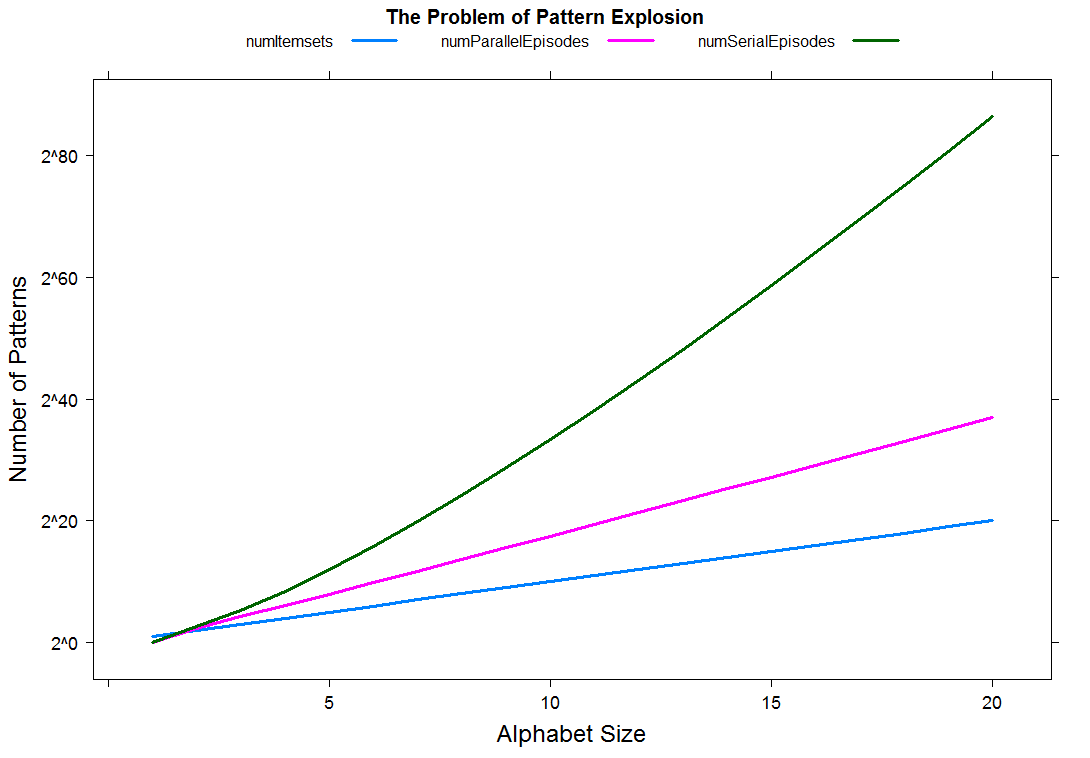
\includegraphics[width=0.75\textwidth]{patternExplosion}
	\caption{Number of patterns for Different Alphabet sizes. For each observation in this plot the maximal length of the episode patterns $m$ was set to the same value as the alphabet size to allow for a comparison with the number of frequent itemsets.}
	\label{fig_patternExplosion}
\end{figure}

Note that the scale of the y-axis is logarithmic, which shows that the number of possible episode patterns greatly exceeds the number of possible itemsets. This is practical information when choosing support thresholds for episode pattern mining algorithms, 
\chapter{Suggested Algorithms}
\label{chapter_solutions}

% **************************** Define Graphics Path **************************
\ifpdf
    \graphicspath{{Chapter4/Figs/Raster/}{Chapter4/Figs/PDF/}{Chapter4/Figs/}}
\else
    \graphicspath{{Chapter4/Figs/Vector/}{Chapter4/Figs/}}
\fi

This chapter presents the suggested learning algorithms for predictive models in detail. Section \ref{sec_predictiveEpisodeMining} explains predictive episode mining, an approach that aims to discover predictive episodes in the stream. Section \ref{sec_FeatureBasedStreamWindowClassification} explains the idea of feature based stream window classification in order to predict event occurrences. 

\section{PERMS - Predictive Episode Rule Mining in Streams}
\label{sec_predictiveEpisodeMining}
The first suggested algorithm is called the PERMS algorithm, short for \textbf{P}redictive \textbf{E}pisode \textbf{R}ule \textbf{M}ining in \textbf{S}treams.

\subsection{Basic Ideas and Definitions}
In order to fully explain the algorithm we first need to define what we mean by predictive episode rules.

\begin{mydef}
\label{def_predictiveEpisode}
\textbf{Predictive Episode Rule} An episode $\alpha$ is called a predictive episode rule for event $A \in \Sigma$ if $\alpha$ has the form $\beta \rightarrow A$ where $\beta$ is an episode. 
\end{mydef}

In the context of a predictive episode rule $\alpha = \beta \rightarrow A$ we also refer to $\beta$ as the prefix and to $A$ as the suffix or target event of $\alpha$.
The basic idea of the prediction algorithm using predictive episode rules is rather simple. If given a set $P$ of predictive episode rules, we monitor the stream and whenever we detect the prefix of an episode in $P$ we predict an occurrence of $A$. The idea is similar to the mining of sequential rules or rule-based classification (TODO: cite). In principle $A$ does not need to be a single event label but could also be a more complex structure, like an episode. In this thesis we restrict ourselves to single events as suffixes for predictive episode rules.
Of course there is an infinite amount of predictive episode rules for an event type, finding those predictive episode rules that are actually useful for predicting the occurrence of an event is the main task when building (training) the model. The use case here is very similar to the related work that deals with the constraint based mining of episode rules (TODO: cite), where episode rules are mined in order to discover dependencies between earthquakes. There are two main important differences that make the approach used by the authors (TODO: name them) impractical.

\begin{itemize}
 \item We are interested in episode rules of one specific type (those predicting the desired event $A$), thus it is not necessary to mine all frequent episode rules in the stream.
 \item We are dealing with data in a streaming environment, meaning we can neither analyze the whole data, nor make multiple passes over the entire stream.
\end{itemize}

In order to describe how the set $P$ is built by the suggested learning algorithm,we first need to define frequency, support and confidence for predictive episode rules, which are similar to classic association rules(TODO: cite). Before this can be done however we need to determine which frequency definition we will use in this algorithm. 

\subsection{Choice of Frequency Measure}

Recall that there are three main frequency measures that were proposed in the literature:

\begin{itemize}
	\item The Window-based Frequency (see defintion \ref{def_windowBasedFrequency})
	\item The frequency based on minimal occurrences (see definition \ref{def_minimalOccuranceFrequency})
	\item The frequency based on non-overlapping occurrences (see definition \ref{def_nonOverlappingFrequency})
\end{itemize}

Their properties were already discussed in subsection \ref{subsec_otherFrequency}. While the frequency measure using the non-overlapping occurrences is the latest measure and offers the best theoretical runtime, when recognizing episodes in a sequence it has a few drawbacks that are detrimental to its use in the given scenario. The first one is that it does not limit the duration of the episode occurrences. However limiting the duration of episode rules, or in other words giving episode occurrences expiry times (TODO: cite) is necessary when predicting event occurrences in streams. Consider for example the simple predictive episode rule $\alpha = B \rightarrow A$ and the following example sequence: 

\begin{equation}
S = [ (B,1),(C,2),(A,3),(B,4),...,(A,2000) ] 
\end{equation}

The non-overlapping frequency definition recognizes both $(B,1) \rightarrow (A,3)$ and $(B,4) \rightarrow (A,2000)$ as equally valid occurrences of $\alpha$ in $S$. However it is to be expected that when looking for episode rules for predictive purposes in a stream the events should happen close to each other (time-wise). This means that in this case $(B,1) \rightarrow (A,3)$ is likely a correct occurrence and prediction, whereas the occurrence $(B,4) \rightarrow (A,2000)$ is simply owed to the fact that at some point of time event $A$ will occur again in the stream and $(B,4)$ happened to occur a long time before that, without there necessarily being a correlation or causality.
Additionally the non-overlapping frequency assumes that there is one long sequence, from which the episodes are to be mined. The window-based frequency however works on a set of individual windows of a sequence or stream. In the previous work this had not been an advantage or disadvantage, since it did not focus on the streaming scenario, which meant that it was possible to analyze the entire sequence. This lead to the use of sliding windows over the sequence when using the window-based frequency. In the streaming scenario it is impossible to use all of the data, instead a certain selection is necessary. This can be done easily when using the window-based frequency by simply storing the windows that are of interest. Selecting data for the non-overlapping frequency definition is more difficult. Thus we will use the window-based frequency in this approach

\subsection{Basic Definitions}
Since we decided on a frequency measure it is now possible to define frequency, support and confidence of predictive episode rules.

\begin{mydef}
\label{def_frequency}
\textbf{Frequency} If given a set of time windows $WIN$ (see definition \ref{def_timeWindow}) of a sequence or stream the frequency of a predictive episode $\alpha$ is defined as the number of windows in which $\alpha$ occurs: $freq(\alpha) = |\{W\,|W \in WIN\; \land \alpha\; occurs \; in \; W\}|$
\end{mydef}

\begin{mydef}
\label{def_support}
\textbf{Support} If given a set of time windows $WIN$ of a sequence the support of a predictive episode $\alpha$ is defined as $s(\alpha) = \frac{freq(\alpha)}{|WIN|}$ TODO: source
\end{mydef}

\begin{mydef}
\label{def_confidence}
\textbf{Confidence} The confidence of a predictive episode $\alpha = \beta \rightarrow A$ is defined as $c(\alpha) = \frac{freq(\alpha)}{freq(\beta)}$ TODO: source
\end{mydef}

The intention is clear and similar to the mining of classic association rules (TODO: cite): If a rule has a high confidence, it means that the prefix of the rule rarely occurs without its suffix $A$, meaning there is a high chance that this is a true predictor for the event $A$. Thus the goal of PERMS is to find a set of predictive episode rules $P$ that have a very high confidence and are above a certain support limit.

\subsection{Choice of training data}
Recall that in streaming applications it is impossible for to analyze the whole stream as one sequence using multiple passes. Thus, when presented with a stream any prediction or forecasting algorithm first needs to take some time to study the stream and extract training data to build the model. So if given an annotated event stream, how do we determine the training data? As it was described in section \ref{sec_episodeMiningBackground} the data basis for episode mining is one very long sequence. Thus the first simple approach would be to simply record the stream as a sequence until we have reached a number of desired elements or run out of memory. The recorded sequence would then be the training sequence from which the predictive episode rules can be mined. This approach is visualized in figure \ref{fig_trainingDataNaive}.

\begin{figure}[h]
	\centering
  	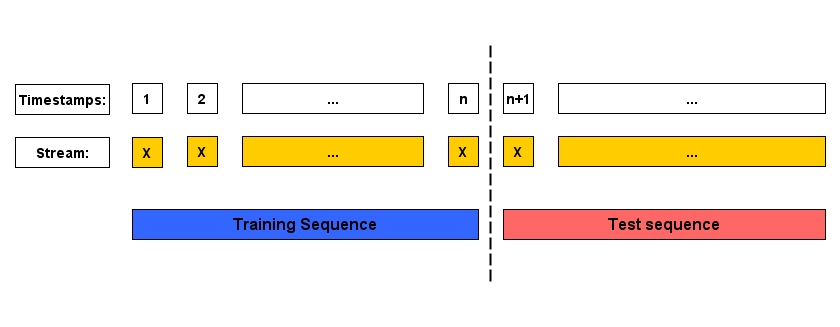
\includegraphics[width=\textwidth]{trainingDataNaive}
	\caption{Visualization of a simple split of the stream into a training segment at the beginning, followed by a (potentially endless) test phase}
	\label{fig_trainingDataNaive}
\end{figure}

The disadvantage of this naive approach is that there is no guarantee about the number of occurrences of the event we aim to predict. Say we want to predict $A$ and $A$ is rather sparse in the beginning of the stream, then we will have a very small data basis to extract predictive episode rules for $A$ and thus will likely not succeed. 
A better approach is to scan the stream for occurrences of the event $A$ and whenever an event of type $A$ enters the window we store the current window in a list until we have a sufficient number of windows. This approach is visualized in figure \ref{fig_trainingDataWindowsOfA}. This approach guarantees that we have a sufficient number of windows that are immediately followed by the target event. The mining process then is to simply find frequent episodes in the mined windows. Each of these then automatically corresponds to the prefix of a potential predictive episode rule with the suffix being the target event ($A$ in the figures).

\begin{figure}[h]
	\centering
  	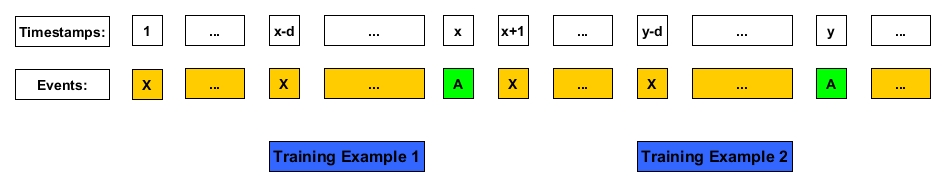
\includegraphics[width=\textwidth]{trainingDataWindowsOfA}
	\caption{Visualization of using fixed windows that precede the target event as training examples. Predictive episodes can be mined from the windows that are extracted from the stream as shown above.}
	\label{fig_trainingDataWindowsOfA}
\end{figure}

The obvious and very big disadvantage is that there are no negative examples in the training sample taken from the stream. Each window is immediately followed by the target event $A$, thus every episode mined from the windows can have $A$ appended as a suffix and thus every predictive episode rule will have a confidence of $1.0$. This means that selection via confidence is meaningless, since we have seen no negative examples, meaning windows that are not followed by $A$. However negative examples can be extracted from the stream in a similar manner. This is the basic idea behind the training data selection in PERMS. It is visualized in figure \ref{fig_trainingDataPositiveAndNegativeWindows}. 

\begin{figure}[h]
	\centering
  	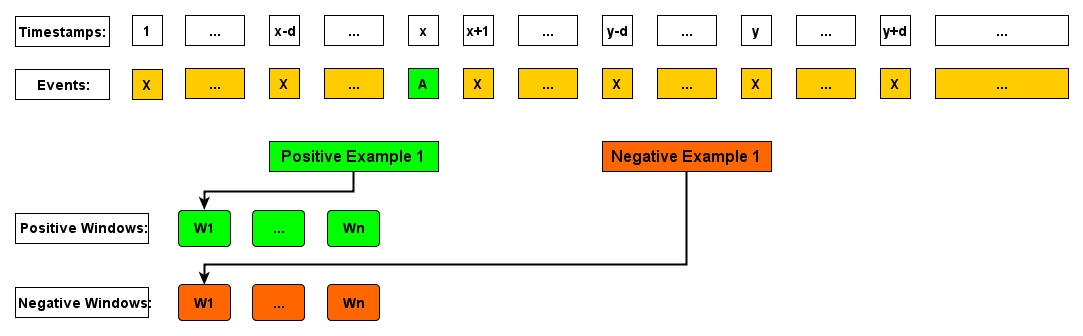
\includegraphics[width=\textwidth]{trainingDataPositiveAndNegativeWindows}
	\caption{Extracting positive and negative example windows from the stream.}
	\label{fig_trainingDataNaive}
\end{figure}

There are still some issues with this approach that can be detrimental to the predictive performance of the model. One issue is that, in the simple standard scenario extract an equal amount of positive and negative windows from the stream with no respect to the original distribution. If $A$ occurs very rarely, having an equal amount of positive and negative examples in the training data does not reflect the original event distribution in the stream. If that is the case, this can be fixed by including a number of negative examples that is proportionate to the original distribution (which is either known or learned while extracting the training data). However it is unclear if that would actually have a significantly positive effect on the performance of the resulting model.



TODO: define negative and positive windows!




\subsection{PERMS Parameters and Pseudocode}

The PERMS algorithm uses the following user-defined parameters:

\begin{itemize}
	\item \textbf{$d$} - the (temporal) size of the sliding window. This also implies that all windows which the predictive episode rules will be mined from will exactly have duration $d$. TODO: talk about episode duration?	
	\item \textbf{$m$} - the number of windows to mine the predictive episode rules from. Basically the sample size we take from the stream.
	\item \textbf{$s$} - the minimum support that predictive episode rules must have to be considered for the model (rules with support $s$ or higher are frequent).
	\item \textbf{$|P|$} - the desired size of the final set of predictive episodes.
\end{itemize}


The basic idea of the PERMS algorithm is the following:
We start at the beginning of the stream and keep a sliding window of a user defined size $d$ in memory. Whenever an event of type $A$ enters the window we store the current window in a list until we have a sufficient number of windows ($m$). Additionally we also store $m$ windows that do not contain $A$ and were also not followed by $A$ in the near future. Once we have enough windows, we can start to mine serial and parallel episodes from the windows preceding $A$ that have support $s$ or higher. For that purpose we employ the apriori-like algorithms mentioned in TODO. Afterwards we rank the discovered rules by confidence, keep the $|P|$ episodes with the highest confidence and return them as the set of predictive episodes $P$.
The subsequent application of the predictive model to the stream is very simple: If an episode $\alpha \in P$ occurs in the current sliding window output $1$ and otherwise output $0$ for the current sliding window.
TODO: pseudocode


\section{Feature Based Stream Window Classification}
\label{sec_FeatureBasedStreamWindowClassification}

The basic idea of the second approach called feature based stream window classification is similar to the one of perms. In fact the process of gathering training data as visualized in figure \ref{trainingDataPositiveAndNegativeWindows} is exactly the same. 


\section{Evolving the models with the stream}
\chapter{Proof of Concept}
\label{chapter_proofOfConcept}

% **************************** Define Graphics Path **************************
\ifpdf
    \graphicspath{{Chapter5/Figs/Raster/}{Chapter5/Figs/PDF/}{Chapter5/Figs/}}
\else
    \graphicspath{{Chapter5/Figs/Vector/}{Chapter5/Figs/}}
\fi

This chapter describes the steps taken to implement the algorithms presented in chapter \ref{chapter_solutions}, as well as the data gathering and pre-processing steps necessary to evaluate the algorithms, as presented in chapter \ref{chapter_evaluation}.

\section{Choice of Programming language}
While the algorithms can in theory be implemented in any programming language the programming language has, apart from personal preferences, implications on the usability of the algorithms. As a language java was chosen, due to the following reasons: There are multiple useful streaming and machine learning frameworks such as Apache Spark \cite{meng2016mllib} or Apache Flink \cite{carbone2015apache} which are also available for java. This means that the frameworks can be used in the implementation, eliminating the need to re-implement functionality like feature-based classifiers or build interfaces to other programming languages that provide such functionality (like R). Future Work can integrate the algorithms into the stream processing frameworks in order to make use of the scalability of their architecture.

\section{The Implementation}

The algorithms were implemented as an eclipse Mars project using java 8. Dependencies to other projects are handled via the build-tool Maven. 

\subsection{Package Structure}

In the following the packages and subpackages are listed and briefly described.

\begin{itemize}
	\item \textbf{data} Main package for basic data representation, data gathering and basic operations on data.
	\begin{itemize}
		\item \textbf{data.crawling} contains classes for gathering raw data from the web-source
		\item \textbf{data.events} contains classes for basic event representations
		\item \textbf{data.stream} contains classes and interfaces for data streams, which can either be completely loaded into memory or read incrementally from files.
		\item \textbf{data.synthetic} contains a partial implementation of the sequence generator as suggested by Zimmermann et al. \cite{zimmermann2012generating}. This can be used to generate artificial data with specific episodes in order to test mining algorithms on it.
		\item \textbf{transformation} contains classes that implement data extraction and transformation utilities, such as extracting numerical time series from the raw data, and transforming the numerical time series to a categorical event stream.
	\end{itemize}
	\item \textbf{episode} Main package for episode patterns
	\begin{itemize}
		\item \textbf{episode.pattern} Main package for the episode patterns used in the thesis and evaluation.
		\begin{itemize}
			\item \textbf{episode.pattern.mining} contains classes implementing the general episode mining algorithm as specified in algorithm \ref{alg_generalEpisodeMining} as well as the candidate generation procedures for serial and parallel episodes as described in section \ref{sec_candidateGen}
			\item \textbf{episode.pattern.recognition} contains classes implementing the episode recognition algorithms as described in algorithms \ref{alg_SerialEpisodeDetection} and \ref{alg_ParallelEpisodeDetection}.
			\item \textbf{episode.pattern.storage} contains classes implementing episode tries for efficient storage of episodes. Also see section \ref{sec_episodeTrie} for more details on how the data structure works.
		\end{itemize}
		\item \textbf{episode.unstable\textunderscore experimental\textunderscore lossy\textunderscore counting} Package that contains experimental, less sophisticated classes to experiment with episode mining using the lossy counting algorithm. The contents of this package were not used to generate any final results as presented in chapter \ref{chapter_evaluation}.
	\end{itemize}
	\item \textbf{evaluation} contains classes that evaluate predictive models and serialize the results
	\item \textbf{experiment} main package for experiment execution and runs of the complete framework (meaning training, testing and evaluating models)
	\item \textbf{prediction} Main package for predictive models and training procedures
	\begin{itemize}
		\item \textbf{prediction.training} contains classes that extract training examples and provide utilities for model training
		\item \textbf{prediction.models} contains the model classes for all types of predictive models
	\end{itemize}		
	\item \textbf{semantics} contains all functionality to access the Dbpedia \cite{auer2007dbpedia} or provide semantic knowledge in other forms.
	\item \textbf{util} contains utility classes such as standard formatters and helpful IO functionality.
\end{itemize}

\subsection{The Dependencies}
The project is realized as a maven project that has a few dependencies to other projects, these are:

\begin{itemize}
	\item \textbf{junit}: For unit testing purposes
	\item \textbf{apache-jena-libs}: Dependency to access the dbpedia via SPARQL-queries in order to use semantic knowledge.
	\item \textbf{quartz} and \textbf{quartz-jobs}: Open-source library for automatic process execution and scheduling (used in the data gathering process). Java does have built-in solutions for this, such as the \textit{ScheduledExecutorService-class} but the scheduler for processes sometimes terminated, seemingly without reason and stopped starting scheduled processes. The solution using the quartz-library does not suffer from these problems.
	\item \textbf{spark-core} and \textbf{spark-mlib}: Dependency to the apache spark library \cite{meng2016mllib}, a library for distributed big-data processing and machine learning. The library is used for its random forest implementation (which could easily be exchanged for another feature-based classifier) to use with the FBSWC algorithm.
\end{itemize}

\subsection{Basic Class Interactions}
The interactions between the classes are best explained separately for model training and evaluation. The class diagram depicted in figure \ref{fig_classDiagramTraining} shows the core classes that interact while training the models.

\begin{figure}[h]
	\centering
  	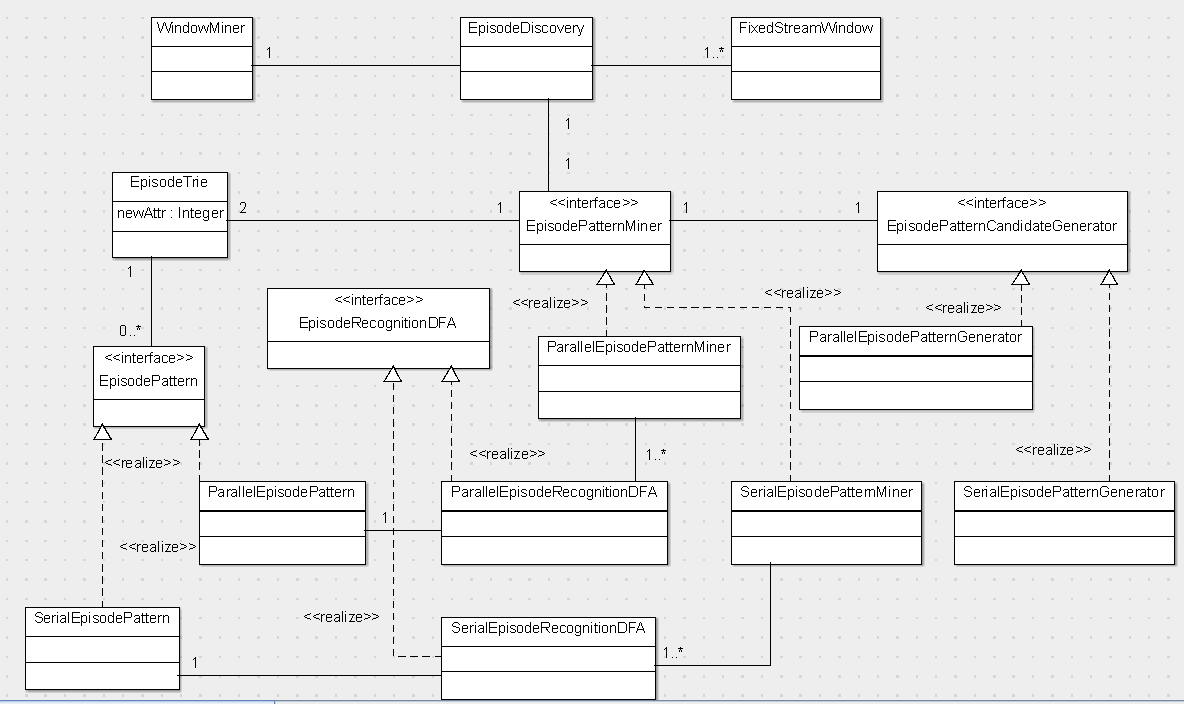
\includegraphics[width=\textwidth]{classDiagramTraining}
	\caption[Class Diagram: Training Phase]{Class diagram of the most important classes during the training of predictive models.}
	\label{fig_classDiagramTraining}
\end{figure}

The central class is called \textit{EpisodeDiscovery}, which makes use of the \textit{WindowMiner} to obtain the training examples, which it then provides as input to the pattern miners. In addition to the training examples the pattern miners requires:

\begin{itemize}
	\item A candidate generator, meaning either a \textit{ParallelEpisodePatternGenerator} or a \textit{SerialEpisodePatternGenerator}
	\item The \textit{EpisodeTrie} as a data structure to efficiently store episodes (see section \ref{sec_episodeTrie} for a detailed explanation)
	\item A deterministic finite automaton for each episode in order to recognize it in the windows of the stream. 
\end{itemize}

Note that there are general interfaces provided, whose concrete implementations will be chosen depending on which kind of episodes are supposed to be mined (either serial or parallel). The main class interactions during the evaluation of the models is visualized in figure \ref{fig_classDiagram1}.

\begin{figure}[h]
	\centering
  	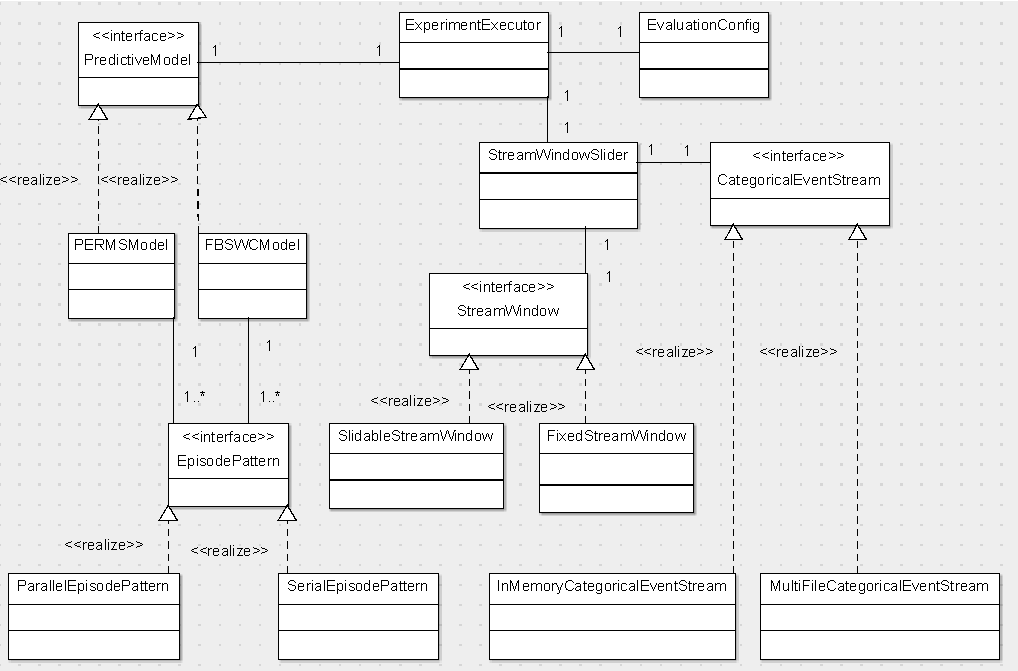
\includegraphics[width=\textwidth]{classDiagram1}
	\caption[Class Diagram: Test Phase]{Class diagram of the most important classes during the evaluation of predictive models.}
	\label{fig_classDiagram1}
\end{figure}

In order to evaluate constructed models, the \textit{ExperimentExecutor}-class plays the central role. It makes use of the configuration to properly initialize the models and uses the \textit{StreamWindowSlider}-class to iterate over the different stream windows of the underlying categorical event stream. Both model classes use the mined episode patterns to compute their predictions. Once again there are multiple implementations of some interfaces, allowing either for the stream to be kept in memory or to be continuously read from files as well as for the time windows to be fixed or slidable. 

\section{Efficient Episode Storage}
\label{sec_episodeTrie}
The naive way of storing episodes is to store each episode as a list of event types, which are sorted in alphabetical order in case of parallel episodes and according to the ordering function in case of serial episodes. This however means that each episode of length $l$ will require $\Theta(l)$ memory, which is not a lot for an individual episode but adds up when large numbers of episodes need to be kept in memory, which is the case in frequent episode mining. \\
Organizing the episodes in a trie-like data structure can greatly reduce the amount of memory needed for sets of episodes if many of these episodes have common prefixes. This idea was already put to use by Baumgarten et al. when mining sequences of sets from large sequences \cite{baumgarten2003tree}. \\
There are two types of tries: Tries for parallel episodes and tries for serial episodes. Both can be treated in exactly the same way by algorithms if the events of parallel episodes are ordered in an arbitrary but fixed order (for example alphabetically according to the event type names). In case of serial episodes the ordering is kept according to the ordering function. Figure \ref{fig_trieExample} visualizes the storage of episodes in tries. 
\begin{figure}[h]
	\centering
  	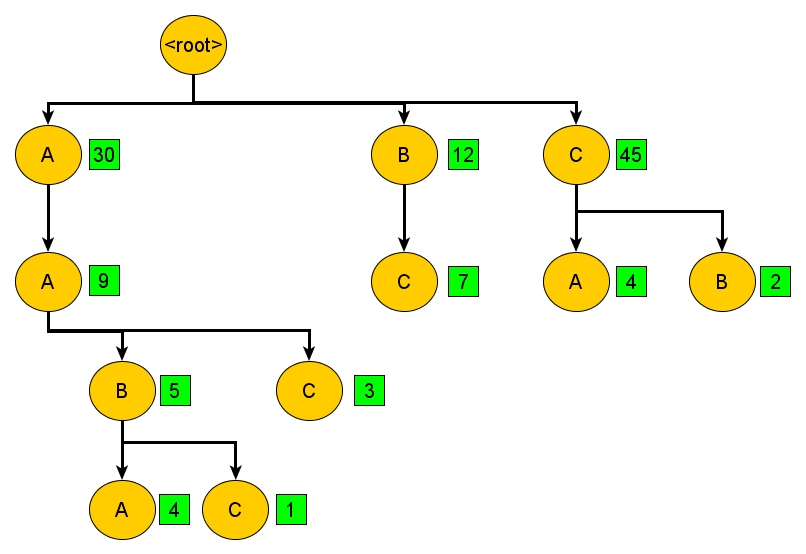
\includegraphics[width=0.75\textwidth]{trieExample}
	\caption[Episode Trie for Serial Episodes]{An example of an episode trie storing serial episodes. The yellow nodes are the nodes of the trie, each one is representing an episode. The green boxes represent the value associated with that episode, which could for example be the frequency as returned by the counting algorithms.}
	\label{fig_trieExample}
\end{figure}

The trie consists of an artificial root node, which has all episodes of length $1$ as child-nodes. Each level $i$ of the tree stores all episodes of exactly length $i$ (with the root node being level $0$). An episode is uniquely identified by a node in the tree, the whole episode can be reconstructed by walking backwards to the root of the tree. The advantage is clear: if there are episodes with the same prefix, such as $A \rightarrow A \rightarrow B \rightarrow A$ and $A \rightarrow A \rightarrow B \rightarrow C$ the prefix only needs to be stored once. Furthermore episode-frequency fulfills the a-priori criterium, which means that if an episode is present in the trie while mining frequent episodes, all its subepisodes (which are prefixes of that episode) will be present in the trie as well. Tries for parallel episodes have exactly the same structure, except that after having visited a node that is annotated with a certain event type $X$, event types that rank lower in the alphabetical order than $X$ can no longer follow.

\chapter{Conclusion and Future Work}
\label{chapter_conclusion}

% **************************** Define Graphics Path **************************
\ifpdf
    \graphicspath{{Chapter6/Figs/Raster/}{Chapter6/Figs/PDF/}{Chapter6/Figs/}}
\else
    \graphicspath{{Chapter6/Figs/Vector/}{Chapter6/Figs/}}
\fi
%\chapter{Conclusion and Future Work}
\label{chapter_conclusion}

% **************************** Define Graphics Path **************************
\ifpdf
    \graphicspath{{Chapter7/Figs/Raster/}{Chapter7/Figs/PDF/}{Chapter7/Figs/}}
\else
    \graphicspath{{Chapter7/Figs/Vector/}{Chapter7/Figs/}}
\fi

This thesis studied the mining of complex events in data streams and how these events can be used in order to build predictive models for the data stream. In particular, the focus was put on very specific complex events called episodes, which are complex event patterns that are formed by combining basic events using the sequence or the conjunction operator. For the purpose of prediction, two algorithms were developed and implemented to train predictive models for categorical events in streams: \textbf{P}redictive \textbf{E}pisode \textbf{R}ule \textbf{M}ining in \textbf{S}treams (PERMS) and \textbf{F}eature \textbf{B}ased \textbf{S}tream \textbf{W}indow \textbf{C}lassification (FBSWC). Both algorithms mine the categorical event stream for training data and subsequently mine frequent serial and parallel episodes from them. PERMS then constructs an ensemble of predictive episode rules to predict the target event, while FBSWC trains a feature based classifier using the occurrences of episodes as features. \\
The evaluation on financial data streams was able to show that both algorithms can produce useful predictive models, which interestingly predict most of the extreme events (large increases or decreases in stock value) correctly. On average however, the predictive performance of the produced models is largely indistinguishable from random guessing and worse than a simple moving average, which means that, at least for the domain of financial data streams, the methods still need to be improved. However, the fact that many configurations show outliers with accuracy greater than 65\% shows that the algorithms are in fact able to build well performing models. The evaluation also showed that the addition of semantic knowledge can improve model accuracy in some cases but significantly increases the training time, since there are more patterns that need to be considered.\\
There are many future work opportunities in this area. First of all, it would be interesting to do an in-depth analysis of why the models produced by PERMS and FBSWC correctly predict many of the extreme increases or decreases in stock value. Finding out whether this is due to chance or whether the models actually found rules that allowed them to correctly predict the extreme cases would be very valuable information for refining the algorithms. Secondly, PERMS and FBSWC should be evaluated with data from other domains to see if the weak average performance in terms of accuracy is domain specific. Additionally the inclusion of semantic knowledge could be extended and more extensively evaluated as the evaluation has shown that additional events that are derived from semantic knowledge, can improve the predictive performance of the trained models. Furthermore, the suggested modifications to the algorithms as suggested in section \ref{sec_EvolvingModels} could be implemented and the effect of evolving models as the stream progresses could be studied in more detail. The predictive performance of evolving models could then be compared to the static case. While episode mining in streams has received attention, there are still many open problems, such as mining general episode patterns in data streams. Solutions to these open problems could contribute to an even larger set of possible patterns that can be mined, increasing the chance to find helpful correlations or rules that help predict events in categorical streams. Apart from that both PERMS and FBSWC could be adapted to work with different kinds of complex event patterns, which might in turn positively impact accuracy.



% ********************************** Back Matter *******************************
% Backmatter should be commented out, if you are using appendices after References
%\backmatter

% ********************************** Bibliography ******************************
\begin{spacing}{0.9}

% To use the conventional natbib style referencing
% Bibliography style previews: http://nodonn.tipido.net/bibstyle.php
% Reference styles: http://sites.stat.psu.edu/~surajit/present/bib.htm

\bibliographystyle{apalike}
%\bibliographystyle{unsrt} % Use for unsorted references  
%\bibliographystyle{plainnat} % use this to have URLs listed in References
\cleardoublepage
\bibliography{References/references} % Path to your References.bib file


% If you would like to use BibLaTeX for your references, pass `custombib' as
% an option in the document class. The location of 'reference.bib' should be
% specified in the preamble.tex file in the custombib section.
% Comment out the lines related to natbib above and uncomment the following line.

%\printbibliography[heading=bibintoc, title={References}]


\end{spacing}

% ********************************** Appendices ********************************

\begin{appendices} % Using appendices environment for more functunality

% ******************************* Thesis Appendix A ****************************
\chapter{How to install \LaTeX} 

\section*{Windows OS}

\subsection*{TeXLive package - full version}
\begin{enumerate}
\item	Download the TeXLive ISO (2.2GB) from\\
\href{https://www.tug.org/texlive/}{https://www.tug.org/texlive/}
\item	Download WinCDEmu (if you don't have a virtual drive) from \\
\href{http://wincdemu.sysprogs.org/download/}
{http://wincdemu.sysprogs.org/download/}
\item	To install Windows CD Emulator follow the instructions at\\
\href{http://wincdemu.sysprogs.org/tutorials/install/}
{http://wincdemu.sysprogs.org/tutorials/install/}
\item	Right click the iso and mount it using the WinCDEmu as shown in \\
\href{http://wincdemu.sysprogs.org/tutorials/mount/}{
http://wincdemu.sysprogs.org/tutorials/mount/}
\item	Open your virtual drive and run setup.pl
\end{enumerate}

or

\subsection*{Basic MikTeX - \TeX~ distribution}
\begin{enumerate}
\item	Download Basic-MiK\TeX (32bit or 64bit) from\\
\href{http://miktex.org/download}{http://miktex.org/download}
\item	Run the installer 
\item	To add a new package go to Start >> All Programs >> MikTex >> Maintenance (Admin) and choose Package Manager
\item	Select or search for packages to install
\end{enumerate}

\subsection*{TexStudio - \TeX~ editor}
\begin{enumerate}
\item	Download TexStudio from\\
\href{http://texstudio.sourceforge.net/\#downloads}
{http://texstudio.sourceforge.net/\#downloads} 
\item	Run the installer
\end{enumerate}

\section*{Mac OS X}
\subsection*{MacTeX - \TeX~ distribution}
\begin{enumerate}
\item	Download the file from\\
\href{https://www.tug.org/mactex/}{https://www.tug.org/mactex/}
\item	Extract and double click to run the installer. It does the entire configuration, sit back and relax.
\end{enumerate}

\subsection*{TexStudio - \TeX~ editor}
\begin{enumerate}
\item	Download TexStudio from\\
\href{http://texstudio.sourceforge.net/\#downloads}
{http://texstudio.sourceforge.net/\#downloads} 
\item	Extract and Start
\end{enumerate}


\section*{Unix/Linux}
\subsection*{TeXLive - \TeX~ distribution}
\subsubsection*{Getting the distribution:}
\begin{enumerate}
\item	TexLive can be downloaded from\\
\href{http://www.tug.org/texlive/acquire-netinstall.html}
{http://www.tug.org/texlive/acquire-netinstall.html}.
\item	TexLive is provided by most operating system you can use (rpm,apt-get or yum) to get TexLive distributions
\end{enumerate}

\subsubsection*{Installation}
\begin{enumerate}
\item	Mount the ISO file in the mnt directory
\begin{verbatim}
mount -t iso9660 -o ro,loop,noauto /your/texlive####.iso /mnt
\end{verbatim}

\item	Install wget on your OS (use rpm, apt-get or yum install)
\item	Run the installer script install-tl.
\begin{verbatim}
	cd /your/download/directory
	./install-tl
\end{verbatim}
\item	Enter command `i' for installation

\item	Post-Installation configuration:\\
\href{http://www.tug.org/texlive/doc/texlive-en/texlive-en.html\#x1-320003.4.1}
{http://www.tug.org/texlive/doc/texlive-en/texlive-en.html\#x1-320003.4.1} 
\item	Set the path for the directory of TexLive binaries in your .bashrc file
\end{enumerate}

\subsubsection*{For 32bit OS}
For Bourne-compatible shells such as bash, and using Intel x86 GNU/Linux and a default directory setup as an example, the file to edit might be \begin{verbatim}
edit $~/.bashrc file and add following lines
PATH=/usr/local/texlive/2011/bin/i386-linux:$PATH; 
export PATH 
MANPATH=/usr/local/texlive/2011/texmf/doc/man:$MANPATH;
export MANPATH 
INFOPATH=/usr/local/texlive/2011/texmf/doc/info:$INFOPATH;
export INFOPATH
\end{verbatim}
\subsubsection*{For 64bit OS}
\begin{verbatim}
edit $~/.bashrc file and add following lines
PATH=/usr/local/texlive/2011/bin/x86_64-linux:$PATH;
export PATH 
MANPATH=/usr/local/texlive/2011/texmf/doc/man:$MANPATH;
export MANPATH 
INFOPATH=/usr/local/texlive/2011/texmf/doc/info:$INFOPATH;
export INFOPATH

\end{verbatim}



%\subsection{Installing directly using Linux packages} 
\subsubsection*{Fedora/RedHat/CentOS:}
\begin{verbatim} 
sudo yum install texlive 
sudo yum install psutils 
\end{verbatim}


\subsubsection*{SUSE:}
\begin{verbatim}
sudo zypper install texlive
\end{verbatim}


\subsubsection*{Debian/Ubuntu:}
\begin{verbatim} 
sudo apt-get install texlive texlive-latex-extra 
sudo apt-get install psutils
\end{verbatim}

%% ******************************* Thesis Appendix B ********************************

\chapter{Installing the CUED class file}

\LaTeX.cls files can be accessed system-wide when they are placed in the
<texmf>/tex/latex directory, where <texmf> is the root directory of the user’s \TeX installation. On systems that have a local texmf tree (<texmflocal>), which
may be named ``texmf-local'' or ``localtexmf'', it may be advisable to install packages in <texmflocal>, rather than <texmf> as the contents of the former, unlike that of the latter, are preserved after the \LaTeX system is reinstalled and/or upgraded.

It is recommended that the user create a subdirectory <texmf>/tex/latex/CUED for all CUED related \LaTeX class and package files. On some \LaTeX systems, the directory look-up tables will need to be refreshed after making additions or deletions to the system files. For \TeX Live systems this is accomplished via executing ``texhash'' as root. MIK\TeX users can run ``initexmf -u'' to accomplish the same thing.

Users not willing or able to install the files system-wide can install them in their personal directories, but will then have to provide the path (full or relative) in addition to the filename when referring to them in \LaTeX.



\end{appendices}

% *************************************** Index ********************************
\printthesisindex % If index is present

\end{document}
